% Standalone explainer of the PageNet-only system. report.tex and its assets are independent.
% Build: cd paper && latexmk -pdf -interaction=nonstopmode -halt-on-error report.tex
% Evidence: make_results.py and make_figures.py; no test annotations are read by either.
\documentclass[11pt]{article}
\usepackage{fontspec}
\defaultfontfeatures{Ligatures=TeX}
\setmainfont{Latin Modern Roman}
\setmonofont{Latin Modern Mono}[Scale=MatchLowercase,RawFeature={-tlig}]
\usepackage[a4paper,margin=0.95in]{geometry}
\usepackage{amsmath,amssymb,graphicx,booktabs,array,caption,enumitem,xcolor,setspace,placeins}
\usepackage{tikz}
\usetikzlibrary{arrows.meta}
\usepackage[protrusion=true,expansion=true,final]{microtype}
\usepackage[hidelinks,colorlinks=true,linkcolor=black,citecolor=black,urlcolor=blue!55!black]{hyperref}
\hypersetup{pdftitle={Reading Greek Squeezes with Page Networks},pdfauthor={Vasileios Papadimas}}
\usepackage{titlesec}
\setstretch{1.02}
\setlength{\parskip}{0.2em plus 0.1em}
\setlength{\emergencystretch}{2em}
\widowpenalty=10000
\clubpenalty=10000
\setlength{\tabcolsep}{5pt}
\captionsetup{font=small,labelfont=bf}
\setlist{itemsep=2pt,topsep=3pt,parsep=0pt,leftmargin=1.5em}
\renewcommand{\topfraction}{0.8}
\renewcommand{\bottomfraction}{0.7}
\renewcommand{\textfraction}{0.15}
\renewcommand{\floatpagefraction}{0.8}
\definecolor{accent}{HTML}{1F4E79}
\definecolor{subcol}{HTML}{C0392B}
\definecolor{delcol}{HTML}{8E44AD}
\definecolor{inscol}{HTML}{D35400}
\newcommand{\cer}{\mbox{CER}}
\newcommand{\code}[1]{\texttt{#1}}
\newcommand{\Rone}{\textsf{R1}}
\newcommand{\Rtwo}{\textsf{R2}}
\newcommand{\none}{\textit{none}}
\newcommand{\fitwidth}[1]{\resizebox{\ifdim\width>\linewidth\linewidth\else\width\fi}{!}{#1}}
\titlespacing*{\section}{0pt}{1.8ex plus .5ex}{0.8ex}
\titlespacing*{\subsection}{0pt}{1.2ex plus .4ex}{0.5ex}
\titleformat{\section}{\normalfont\large\bfseries\color{accent}}{\thesection.}{0.5em}{}
\titleformat{\subsection}{\normalfont\normalsize\bfseries}{\thesubsection}{0.5em}{}
% Written by paper/make_results.py from the run outputs; do not edit.
\newcommand{\DevOofErrors}{12{,}565}
\newcommand{\DevOofChars}{131{,}473}
\newcommand{\DevOofCer}{9.56\%}
\newcommand{\DevNoMergedErrors}{7{,}935}
\newcommand{\DevNoMergedChars}{96{,}628}
\newcommand{\DevNoMergedCer}{8.21\%}
\newcommand{\DevNestedErrors}{12{,}612}
\newcommand{\DevNestedChars}{131{,}473}
\newcommand{\DevNestedCer}{9.59\%}
\newcommand{\DevNestedAgree}{three}
\newcommand{\DevCombo}{$(\lambda, w, \beta, \nu) = (0.5, 1, 1, 0.8)$}
\newcommand{\DevScoreWeights}{$(\lambda, w, \beta) = (0.5, 1, 1)$}
\newcommand{\DevOpenWeight}{0.6}
\newcommand{\DevNeuralWeight}{0.8}
\newcommand{\DevOpenWeights}{0.3, 0.45, 0.6}
\newcommand{\DevGridPoints}{1800}
\newcommand{\DevNearBest}{43}
\newcommand{\DevSplitGroups}{19}
\newcommand{\DevSplitSqueezes}{48}
\newcommand{\DevSplitErrors}{2{,}072}
\newcommand{\DevSplitChars}{26{,}405}
\newcommand{\DevSplitCer}{7.85\%}
\newcommand{\DevUnsplitSqueezes}{176}
\newcommand{\DevUnsplitErrors}{10{,}631}
\newcommand{\DevUnsplitChars}{105{,}068}
\newcommand{\DevUnsplitCer}{10.12\%}
\newcommand{\DevTrogsErrors}{1{,}464}
\newcommand{\DevTrogsChars}{15{,}862}
\newcommand{\DevTrogsCer}{9.23\%}
\newcommand{\DevTrogsAllErrors}{2{,}128}
\newcommand{\DevTrogsAllChars}{16{,}944}
\newcommand{\DevTrogsAllCer}{12.56\%}
\newcommand{\DevTrogsOptErrors}{1{,}282}
\newcommand{\DevTrogsOptChars}{16{,}052}
\newcommand{\DevTrogsOptCer}{7.99\%}
\newcommand{\ExtLetters}{178.1}
\newcommand{\DeconGram}{15}
\newcommand{\DeconRare}{10}
\newcommand{\DeconDropAt}{5}
\newcommand{\DeconShare}{4\%}
\newcommand{\DeconDropped}{7}
\newcommand{\DeconPublicFound}{5}
\newcommand{\DeconTestFound}{0}
\newcommand{\DeconCutDocuments}{1{,}723}
\newcommand{\DeconCutLetters}{38{,}827}
\newcommand{\DeconCalibPhiDocuments}{173{,}677}
\newcommand{\DeconCalibDocuments}{296}
\newcommand{\DeconCalibSqueezes}{149}
\newcommand{\DeconCalibShare}{91.5\%}
\newcommand{\DeconCalibEditions}{229}
\newcommand{\DeconCalibShareMin}{5.0\%}

\makeatletter
\@for\figname:=teaser,overview_front,relief,registration,detector,neighbourhood,augmentation,tta,confusion,tokens,rows,%
lattice,rover,sweep,squeezes,example\do{\input{figs/\figname.tex}}
\makeatother

\begin{document}
\begin{center}
  {\LARGE\bfseries Reading Greek Squeezes with Page Networks}\\[8pt]
  {\small\textbf{Vasileios Papadimas} --- Athens University of Economics and Business}\\[4pt]
  {\small 10 November 2026}
\end{center}

\begin{abstract}
\noindent A paper squeeze records an inscription as an impression of the carved stone. Its letters appear
in light and shadow, alongside folds, cracks and ornament. We describe a system that reads two photographs
of a squeeze, lit from different directions. It aligns the photographs, combines the visible strokes, and
reads each possible letter together with the marks around it. Models of Greek letter sequences help choose
between uncertain readings; they cannot fill a gap where no letter was detected. Five versions of the
processing chain produce transcripts that are aligned and voted on. We follow the images through these
steps and show both successful readings and remaining errors. The character error rate on confidently
annotated text is \DevNestedCer{} on 224 public squeezes, with each squeeze held out from its reader's training
and from the choice of its weights, and \DevTrogsCer{} for the fixed final output on 50 TROGS-26 test squeezes.
\end{abstract}

\section{What has to be read}
\label{sec:task}
Wet paper pressed into an inscribed stone and dried keeps an impression of the carving. Photographing the
squeeze with light grazing its surface makes the relief visible. The TROGS collection~\cite{howe2025} provides
two such photographs, \Rone{} and \Rtwo{}, with lighting directions roughly a right angle apart. A stroke
across the light shows strongly; one along it may almost disappear. A shadow is therefore evidence about
surface shape, not a dark pixel that can be read as ink. The same light also reveals paper grain, tears,
folds, breaks in the stone and carved ornament.

Figure~\ref{fig:teaser} shows the problem on public squeeze \TeaserSqueeze{}, the \emph{running squeeze}
of later figures. Its rows share the page with wreaths and a paper label. The \emph{reader}, the part of
the system that decides what each mark is (Section~\ref{sec:pagenet}), must find a faint letter without
copying the label or reading the wreath as text.
It must distinguish two questions: \emph{is this region a letter?} and \emph{which letter is it?}
An isolated crop often cannot answer either. The size of the mark, its alignment with a row, a second box
on the same stroke, and the letters around it all matter.

The output has one line per inscription row, without word spaces, translation or restored text.
The dataset writes each Greek letter as one Latin letter:
\begin{center}\setlength{\tabcolsep}{3.2pt}
\begin{tabular}{@{}*{24}{c}@{}}
Α&Β&Γ&Δ&Ε&Ζ&Η&Θ&Ι&Κ&Λ&Μ&Ν&Ξ&Ο&Π&Ρ&Σ&Τ&Υ&Φ&Χ&Ψ&Ω\\
\code{A}&\code{B}&\code{G}&\code{D}&\code{E}&\code{Z}&\code{H}&\code{Q}&\code{I}&\code{K}&\code{L}&\code{M}&
\code{N}&\code{X}&\code{O}&\code{P}&\code{R}&\code{S}&\code{T}&\code{Y}&\code{F}&\code{C}&\code{U}&\code{W}
\end{tabular}
\end{center}
Three signs, \code{\&}, \code{:} and \code{)}, complete its 27 symbols; \code{:} marks an interpunct.
Transcripts in this report use these symbols, as the dataset and its scorer do. Where letter shapes
matter, as in the confusions of Section~\ref{sec:tokens}, letters are written in Greek. Every output
character must come from a detected region and be one of the reader's proposed letters for that region.

We measure errors against the supplied reference transcripts. The main measure, \emph{Core character
error rate} (Core CER), counts missing, wrong and extra characters against confidently annotated text,
including row boundaries. A lower rate is better. Section~\ref{sec:results} explains the scoring and
training exclusions in full.

\begin{figure}[t]
\centering
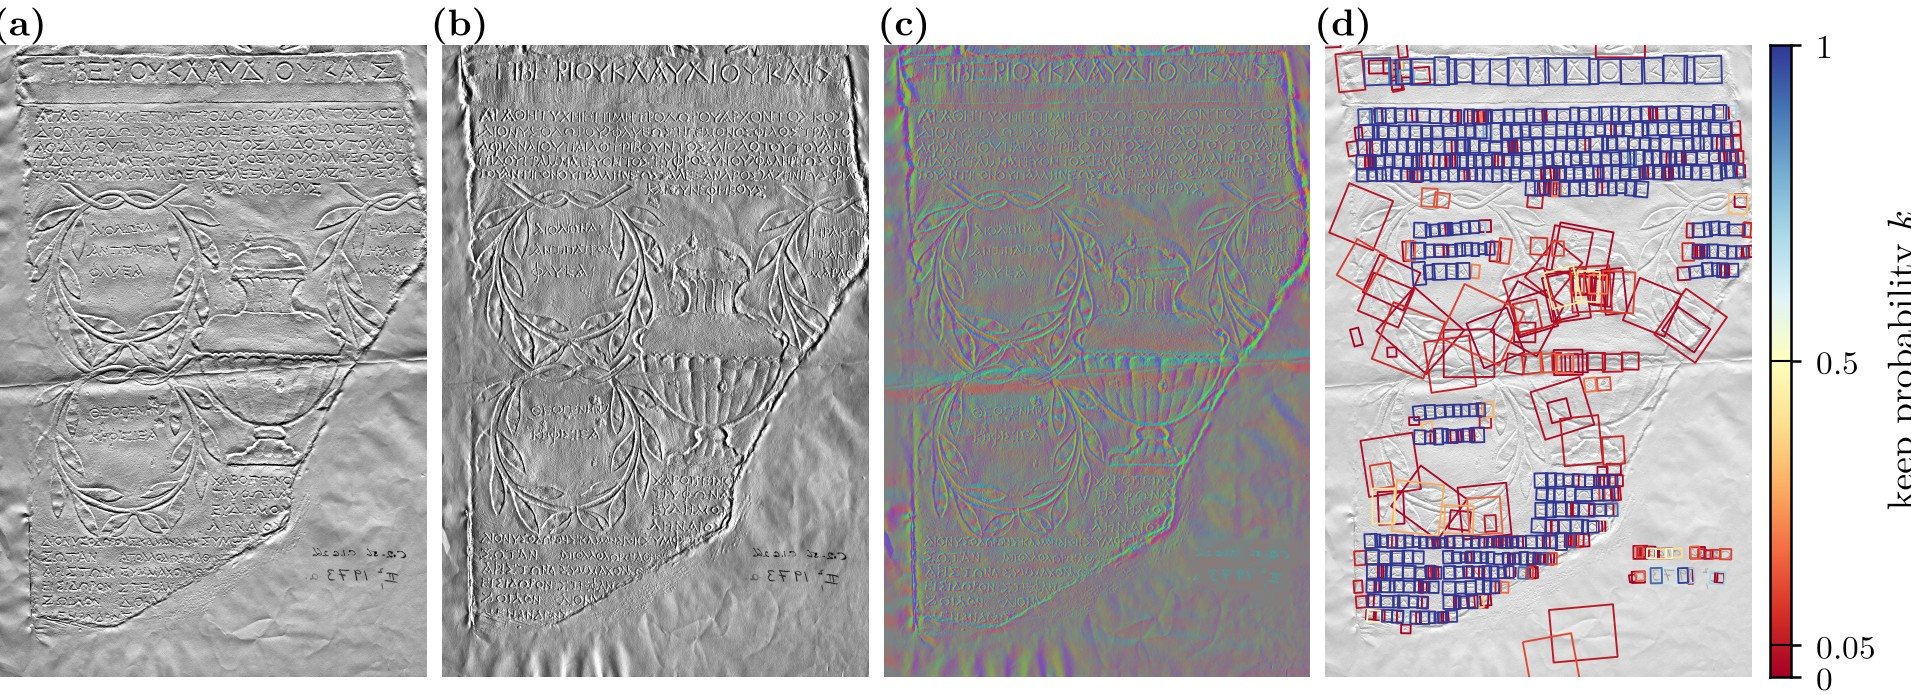
\includegraphics[width=\textwidth]{figs/teaser.jpg}
\caption{\textbf{Letters, folds and ornament under changing light.} Public squeeze \TeaserSqueeze{}.
(a, b)~The two photographs. (c)~The combined relief under three fixed lights, one per colour channel.
(d)~All \TeaserTokens{} candidate boxes, coloured by the reader's probability of keeping them as letters:
blue is high, red low. The ornament attracts many boxes but few accepted letters. This squeeze was
excluded from its reader's training; its \SqueezesShowcaseCer{} Core CER is better than the public average.}
\label{fig:teaser}
\end{figure}

\section{From two photographs to one transcript}
\label{sec:system}
The two photographs cannot simply be overlaid. The paper may have moved or deformed, and stitched scans
may disagree locally. The first task is to align the same piece of paper in both views. Their shadows
then provide two estimates of surface slope, which we render under fixed lights so that the reader sees
a consistent presentation of the strokes (Figure~\ref{fig:overview}).

A \emph{detector} draws a rotated box around each possible letter. We keep its uncertain proposals:
discarding a faint letter here would make it unavailable to the rest of the system. Each box becomes a
\emph{token}: an image crop together with its position, shape and detection scores.

Two \emph{page networks} read these tokens; together they form the reader, whose probabilities combine
both (Section~\ref{sec:training}). Unlike a classifier that sees only one crop, each network also sees
nearby marks and their arrangement on the page. It assigns probabilities to the 27 symbols and to
\none{}, meaning that the box should not contribute a letter. The probability of any letter rather than
\none{} is its \emph{keep probability}, denoted $k$.

The \emph{decoder} turns those probabilities into text. It groups likely letters into rows, lets weaker
marks join nearby rows, and compares possible readings. A reading can use one of a token's proposed
letters or skip that token. Character models, learned from public transcripts and open Greek text, help
rank these alternatives. Repeated names and phrases in the squeeze's other rows provide further context.

On a new squeeze, five separately trained detectors produce five versions of this process, called
\emph{chains}. They share the same page networks and text models, but may find different boxes or align the
images differently. Their complete transcripts are aligned and combined by a vote
(Figure~\ref{fig:overview2}). For public evaluation, we instead use one chain whose models were trained
without the squeeze being read. The public set is divided into five groups, or \emph{folds}, for this purpose.

\begin{figure}[p]
\centering
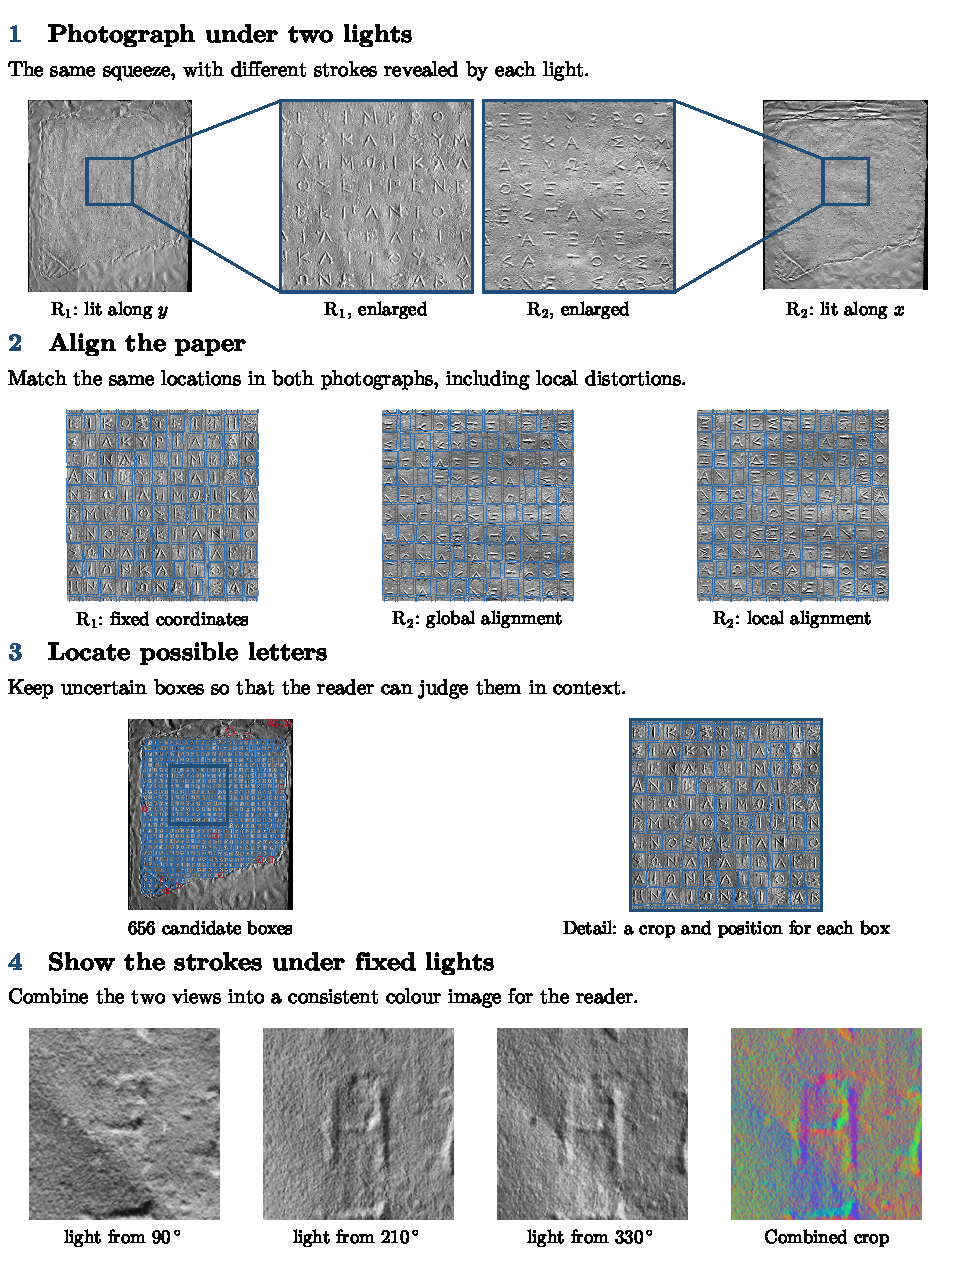
\includegraphics[width=\textwidth]{figs/overview_front.pdf}
\caption{\textbf{From photographs to letter crops.} All images show public squeeze
\OverviewSqueeze{}. The enlargements reveal the different strokes visible under each light.
Alignment brings them into correspondence; detection locates possible letters; relighting combines
their evidence into the colour crop read by the network. Figure~\ref{fig:overview2} continues from here.}
\label{fig:overview}
\end{figure}

\begin{figure}[p]
\centering
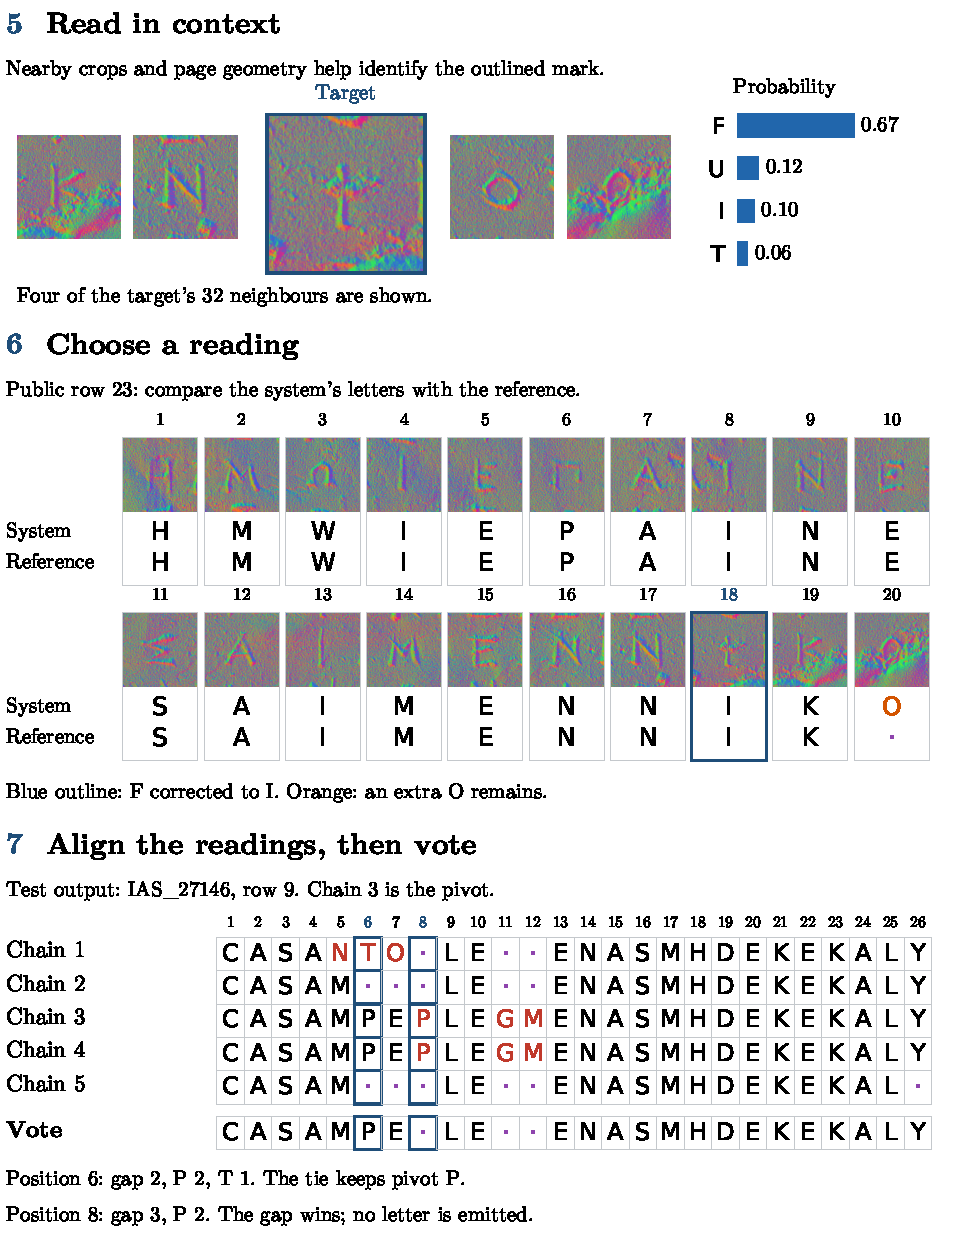
\includegraphics[width=\textwidth]{figs/overview_back.pdf}
\caption{\textbf{From letter crops to a transcript.} Stages 5--6 use public squeeze
\OverviewSqueeze{}; its reference is shown beneath the system's letters. Orange marks an extra output
letter. Stage 7 shows the actual outputs of the five test chains. Each cell is one aligned
position; red marks disagreement with the vote and purple dots are gaps, which emit no letter.
The pivot is the transcript closest to the other four, measured by the total number of edits needed
to align them. Section~\ref{sec:rover} gives the voting rules.}
\label{fig:overview2}
\end{figure}

\section{Aligning the two photographs}
\label{sec:registration}
\subsection{Why brightness cannot simply be matched}
For a locally matte surface with height $h(x,y)$, lit from direction $\phi$ at low elevation $\theta$, the
brightness relative to the surrounding paper is approximately
\begin{equation}
 s=\frac{I}{I_{\mathrm{paper}}}-1
   \approx-\cot\theta\,(\cos\phi\,h_x+\sin\phi\,h_y).
 \label{eq:shading}
\end{equation}
Here $\phi$ is the light's angle in the plane of the paper and $\theta$ its angle above that plane.
The derivatives $h_x$ and $h_y$ describe surface slope in the two image directions.
$I_{\mathrm{paper}}$ is a smooth estimate of the local paper brightness; dividing by it suppresses
broad illumination changes. A photograph measures a directional derivative of height. The two raw images
are therefore not two brightness-preserving views of the same pattern: changing the light changes which
strokes are bright or dark.

In this collection, one view's light runs approximately along $x$ and the other's along $y$. Which is which
is estimated from directional gradient energy. Call their relative shadings $s_x$ and $s_y$. Apart from
scale and sign, they estimate $h_x$ and $h_y$. Differentiate each \emph{across} its light:
\begin{equation}
 \partial_y s_x\ \propto\ h_{xy}\ \propto\ \partial_x s_y.
 \label{eq:mixed}
\end{equation}
The two derivative images now describe the same change in surface slope. Their magnitudes can therefore
guide alignment even where different letters are visible in the two views. This is an approximation:
shadows, non-matte paper and errors in lighting direction need not obey Eq.~\eqref{eq:shading}. The method
checks local image agreement rather than assuming a perfect physical model.

\subsection{Matching the whole page, then local regions}
A coarse detector pass on each view estimates letter scale and offers a map from detected centres. That
map can include a global transformation, separate fits across stitched scans and a smooth local
deformation (a thin-plate spline~\cite{bookstein1989}). But letters visible in one photograph may be missing in the other, so centre
matching alone can accept the wrong correspondence.

A second route registers the mixed-derivative images. Phase correlation searches quarter turns and small
angular offsets; enhanced correlation coefficient alignment~\cite{evangelidis2008} fits Euclidean and affine
maps. Three local levels then refine the map tile by tile, each allowing smaller displacements
(Table~\ref{tab:recipe}). Accepted shifts are fitted with a thin-plate spline, smoothed until its
orientation is preserved. The centre-derived map is also refined with the two finer local levels. Median
tile correlation then selects the best of these three maps. No annotation is used in that selection.
We express all box positions and crops in \Rone{} coordinates and warp \Rtwo{} to match.
This choice makes the implementation asymmetric: the two views are not interchangeable.

Figure~\ref{fig:registration} separates the image-based decision from its evaluation. The map is chosen on
pixels; annotated letter correspondences, available on the public set, independently measure the residual.
Appendix~\ref{app:align} counts the squeezes this improves. A small median residual does not guarantee
that every stitched seam is correct.

\begin{figure}[t]
\centering
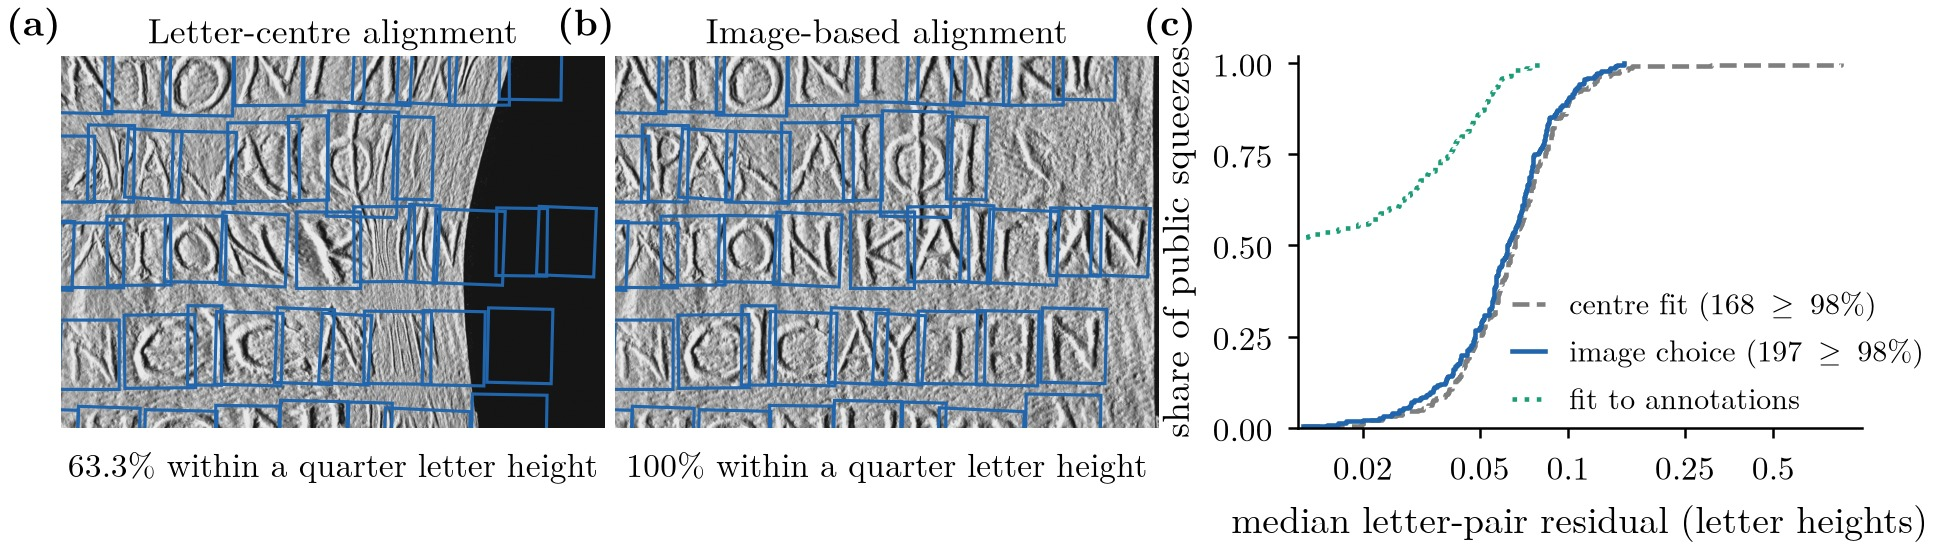
\includegraphics[width=\textwidth]{figs/registration.jpg}
\caption{\textbf{Correcting a local alignment error.} Public squeeze \RegExampleBase{}, in the region where
the two maps disagree most. (a)~Alignment from detected letter centres. (b)~Alignment selected from image
agreement. The boxes stay fixed in \Rone{} coordinates. Over the whole squeeze, the share of annotated
letter pairs within a quarter letter height rises from 63.3\% to 100\%. (c)~Across the public set,
cumulative distributions of median alignment error. The annotation-fitted curve is a reference
comparison only; those correspondences are not supplied to the system. Legend counts use the stricter
98\%-within-a-quarter-height criterion of Appendix~\ref{app:align}.}
\label{fig:registration}
\end{figure}

\section{Combining the light from both views}
\label{sec:relief}
After registration, each shading is normalised by its root mean square on the paper. Mixed derivatives
set the relative sign of the two shadings and support a final tilewise correction of residual alignment.
Their local correlation $\rho$ controls how much of view~2 to trust:
\begin{equation}
 \alpha=\operatorname{clip}\!\left(\frac{\rho-0.1}{0.2},0,1\right),\qquad
 (g_x,g_y)=(\hat s_x,\sigma\alpha\hat s_y)
 \label{eq:gradient}
\end{equation}
when \Rone{} is the $x$-lit view; the attenuated component is exchanged when it is $y$-lit.
$\sigma$ is the relative sign. Where the scans show different paper or cannot be aligned, the representation
falls back to the component supplied by \Rone{}. This avoids combining unrelated strokes, at the cost of
losing the second light there. The absolute groove/ridge ambiguity is resolved by choosing the sign whose
curvature inside confident detections has the profile of carved strokes.

The system uses these slopes directly, without reconstructing the surface's absolute depth.
Three fixed virtual lights, at azimuths $\phi=90^\circ$, $210^\circ$ and $330^\circ$,
produce one image channel each:
\begin{equation}
 r_\phi=-(\cos\phi\,g_x+\sin\phi\,g_y),\qquad
 R_\phi=128+127\operatorname{clip}\!\left(\frac{r_\phi}{4\cdot1.4826\,\operatorname{med}|r_\phi|},-1,1\right).
 \label{eq:relit}
\end{equation}
Each colour channel is one light direction; colour carries no other meaning.
A stroke invisible to one virtual light can show in another.
The rendering standardises the evidence; it does not create relief absent from both photographs.

\begin{figure}[t]
\centering
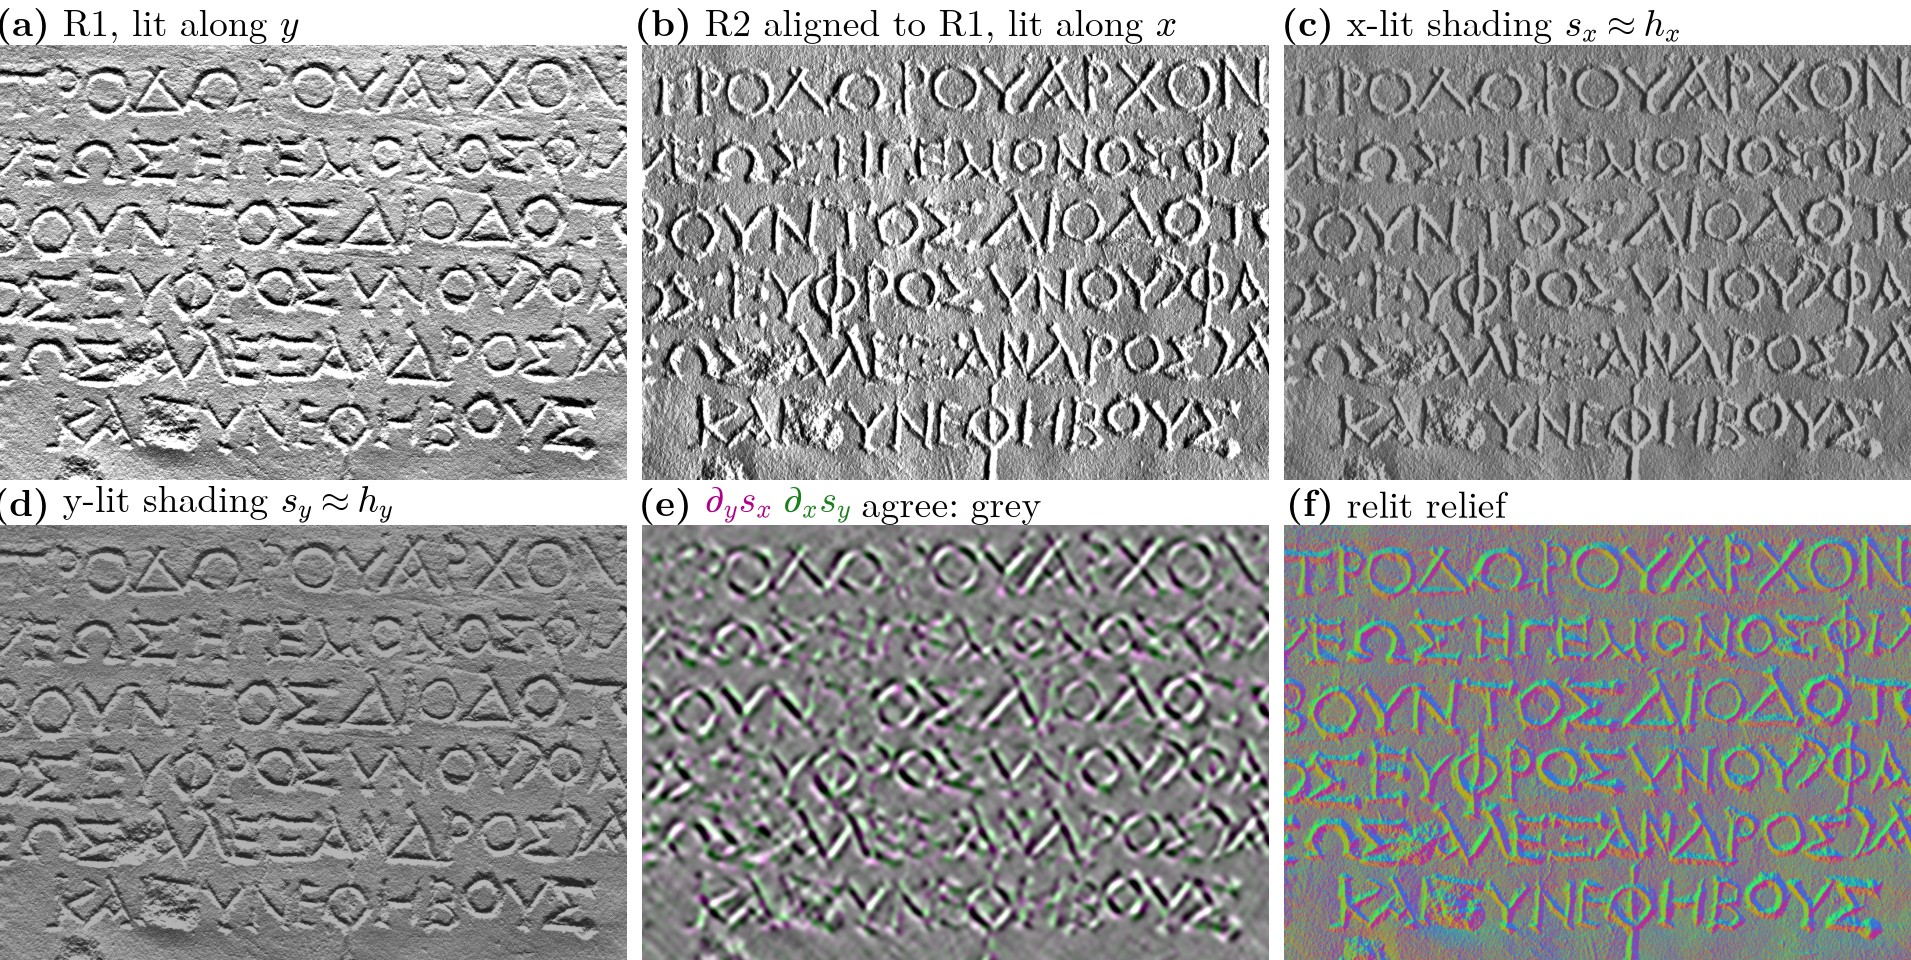
\includegraphics[width=\textwidth]{figs/relief.jpg}
\caption{\textbf{From shadows to a common lighting representation.} A \ReliefWindowWidth{} by
\ReliefWindowHeight{} letter-height window of \TeaserSqueeze{}. (a)~\Rone{}, lit along $y$.
(b)~\Rtwo{} registered onto it, lit along $x$. (c, d)~Their relative shadings: up to scale and sign,
$h_x$ and $h_y$. Grey denotes zero. (e)~The two mixed derivatives: one in magenta, the other in green;
agreement is grey, disagreement tinted. Their correlation is \ReliefWindowAgreement{} in this window
and \ReliefAgreement{} over the page. (f)~The combined field under the three fixed lights.
All panels depict the same paper; the reader's crops are cut from the final panel.}
\label{fig:relief}
\end{figure}

\section{Finding possible letters}
\label{sec:detector}
The detector is YOLO26-L with oriented boxes~\cite{yolo26}, initialised from DOTA aerial-image weights and
fine-tuned for one class: a possible letter. Each of five detectors trains on the portion of the
181-squeeze training set outside its fold. Training includes each view separately and a combined image whose channels are
\Rone{}, registered \Rtwo{} and their pixelwise minimum. Rotation reaches $60^\circ$ and scale ranges from
0.6 to 1.6. A common checkpoint rule selects the weights after training pass (epoch)~59;
details are in Appendix~\ref{app:recipe}.

When reading a page, a coarse pass first measures letter size and refines alignment. The detailed
pass rescales the page to 40-pixel letters and cuts it into $1280\times1280$ tiles with 25\% overlap.
We measure the overlap of two boxes by intersection over union (IoU): the area they share divided by the
area covered by either. Within each tile of one image, rotated non-maximum suppression (NMS) keeps the
better-scoring of two boxes that overlap at IoU above 0.8. A box belongs to its nearest tile centre,
avoiding repeated tile-edge outputs. Detections from the three images are then merged:
weighted box fusion~\cite{solovyev2021} joins boxes at IoU~0.55, and Gaussian soft-NMS~\cite{bodla2017}
reduces the scores of overlapping fused boxes rather than removing them. Each box retains the scores
from the images that found it.

The selected map must govern both the crops and the detections. The detailed pass is therefore repeated
on a page otherwise read from \Rone{} alone, or when at least a tenth of the second view's coarse centres
move by a quarter letter height between the fitted and selected maps (Appendix~\ref{app:align} counts
these pages).

The detector's raw score is not a probability. We calibrate it against observed matches using a monotone
curve (isotonic regression~\cite{zadrozny2002}). Its output, $p_i$, estimates the probability that the box
wins a one-to-one match to an annotated letter at rotated IoU at least 0.5. The curve is fitted using
held-out detections from the other folds. The reader receives $p_i$ as evidence; no box is discarded
for a low $p_i$. The public records contain
\DetectorDetections{} detections for \DetectorLetters{} annotated letters of \Rone{}: \DetectorPerLetter{}
proposals per letter. At least one proposal overlaps \DetectorCoverageClaim{} of the letters at IoU at least 0.3.
Discarding boxes below $p_i=0.5$ would reduce that coverage to \DetectorHalfCoverage{}.
That loss cannot be repaired by a later language model.

\begin{figure}[t]
\centering
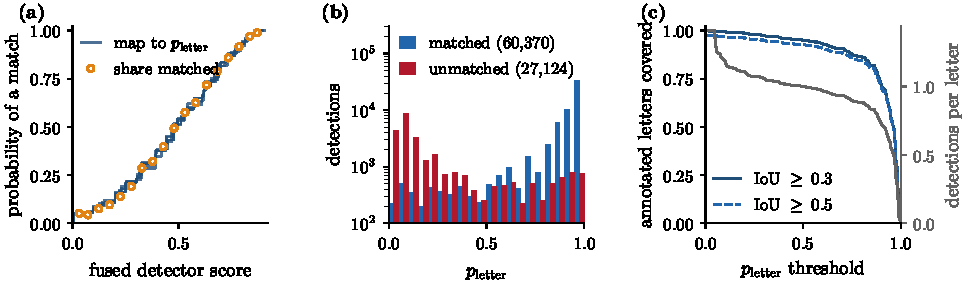
\includegraphics[width=\textwidth]{figs/detector.pdf}
\caption{\textbf{A low detector score need not mean a false letter.} Held-out detections on 224 public
squeezes. (a)~Calibration curves and observed match frequencies. (b)~Scores of matched and unmatched
boxes; unmatched boxes include duplicates. (c)~The fraction of annotated letters reached by at least
one box above a score threshold, at two overlap requirements. Grey shows the number of boxes remaining
per annotated letter. The reader receives all \DetectorDetections{} proposals.}
\label{fig:detector}
\end{figure}

\section{Reading a mark together with its neighbours}
\label{sec:pagenet}
\begin{figure}[t]
\centering
% The page network (fig:pagenet), drawn by hand in TikZ; report.tex inputs it inside the figure.
%
% Left: seven tokens of public squeeze IG_II2_493_Copy1, positions 2-8 of row 23 (cropN.jpg is position N): the crops
% of fig:overview2, stage 6, extracted from figs/overview_back.pdf with `pdfimages -png` (its images 6-12). Their
% first-choice letters are their transcript letters there: that stage outlines the first token of the row whose
% first choice differs (position 18). Regenerating fig:overview2 from other assets does not update them.
% Right: a schematic page, not a squeeze. Token centre (u, v), width, height (letter heights) and tilt (degrees);
% `n` marks the 31 tokens that, with the query at the origin, are its 32 nearest under du^2 + (2 dv)^2. The ellipse
% passes through the 32nd, at 5.55 (the 33rd is at 5.83).
\definecolor{pnimage}{HTML}{2166AC}
\definecolor{pnplace}{HTML}{1B9E77}
\definecolor{pncontext}{HTML}{6A3D9A}
\definecolor{pnmuted}{HTML}{8C8C8C}
\def\pnneighbour{n}
\begin{tikzpicture}[
  x=1cm, y=1cm, line width=0.6pt, font=\footnotesize,
  >={Stealth[length=1.5mm,width=1.2mm]},
  flow/.style={->, draw=black!55},
  block/.style={draw=#1!75!black, fill=#1!12, rounded corners=2pt, align=center, inner sep=2pt},
  vector/.style={draw=#1!75!black, fill=#1!35, rounded corners=0.8pt, minimum width=0.78cm,
                 minimum height=0.28cm, inner sep=0},
  note/.style={font=\scriptsize, align=right, anchor=east, inner sep=0, text=black!80},
  detail/.style={font=\scriptsize, text=black!80},
  place/.style={block=pnplace, anchor=west, align=left, font=\scriptsize, text width=5.68cm, inner sep=2.5pt},
]
% ------------------------------------------------------------------------------------------------ the tokens' path
\node[block=pnimage, anchor=south west, minimum width=7.63cm, minimum height=0.55cm] (encoder) at (2.35, 1.2)
  {\textbf{Crop encoder}\enspace{\scriptsize DINOv3 ViT-S/16}};
\node[draw=pncontext!75!black, fill=pncontext!4, rounded corners=3pt, anchor=south west, minimum width=7.63cm,
      minimum height=1.9cm] (context) at (2.35, 3.0) {};
\node[block=pncontext, minimum width=7.35cm, minimum height=0.55cm] (attention) at (6.165, 3.475)
  {\textbf{Neighbour attention}\enspace{\scriptsize over $N(i)$, 6 heads}};
\node[block=pnmuted, minimum width=7.35cm, minimum height=0.55cm] (ff) at (6.165, 4.425)
  {\textbf{Feed-forward}\enspace{\scriptsize each token alone}};
\foreach \p/\letter [count=\k] in {2/M, 3/W, 4/I, 5/E, 6/P, 7/A, 8/I} {
  \pgfmathsetmacro\x{2.925+(\k-1)*1.08}
  \node[inner sep=0, anchor=south, draw=black!25, line width=0.3pt] (crop\k) at (\x, 0)
    {\includegraphics[width=0.95cm]{diagram/crop\p.jpg}};
  \node[vector=pnimage] (e\k) at (\x, 2.12) {};
  \node[draw=black!55, fill=white, rounded corners=1pt, minimum width=0.78cm, minimum height=0.42cm, inner sep=0,
        font=\ttfamily\small] (out\k) at (\x, 5.35) {\letter};
  \draw[flow] (crop\k.north) -- (\x, 1.2);
  \draw[flow] (\x, 1.75) -- (e\k.south);
  \draw[flow] (e\k.north) -- (attention.south -| \x, 0);
  \draw[flow] (attention.north -| \x, 0) -- (ff.south -| \x, 0);
  \draw[flow] (ff.north -| \x, 0) -- (out\k.south);
}
\draw[line width=1.1pt] (crop4.south west) rectangle (crop4.north east);
\draw[line width=1.1pt] (out4.south west) rectangle (out4.north east);
\node[font=\scriptsize, anchor=north, inner sep=1.5pt] at (crop4.south) {$i$};
\node[font=\scriptsize] at (e4) {$e_i$};
\node[detail] at (6.165, 5.95) {keep $k_i=1-P_i(\none{})$\qquad letter $\pi_i(a)=P_i(a)/k_i$};
% ------------------------------------------------------------------------------------------------ left labels
\node[note] at (2.2, 0.475) {one crop per\\detected box};
\node[note] at (2.2, 2.12) {crop encoding};
\node[note, text=pncontext!75!black, font=\Large] at (2.2, 4.1) {$\times4$};
\node[note] at (2.2, 3.55) {context blocks};
\node[note] at (2.2, 5.35) {$P_i$: 27 symbols\\and \none{}};
% ------------------------------------------------------------------------------------------------ the place
\node[place] (measure) at (10.44, 2.62) {18 measurements $f_i$ $\to$ MLP};
\draw[draw=pnplace!75!black] (2.925, 2.62) -- (9.405, 2.62);
\foreach \k in {1, ..., 7} {
  \node[circle, draw=pnplace!75!black, fill=white, minimum size=0.26cm, inner sep=0] (plus\k) at (e\k |- 0, 2.62) {};
  \draw[draw=pnplace!75!black, line width=0.5pt] (plus\k.north) -- (plus\k.south) (plus\k.east) -- (plus\k.west);
}
\draw[flow, draw=pnplace!75!black] (measure.west) -- (plus7.east);
\node[place] (bias) at (10.44, 3.475)
  {8 pair measurements $f_{ij}$ $\to$ MLP $B$:\\one attention bias per head};
\draw[flow, draw=pnplace!75!black] (bias.west) -- (attention.east);
\begin{scope}[shift={(13.38, 5.4)}, x=0.4cm, y=-0.4cm]
  \fill[black!3, rounded corners=2pt] (-7.35, -2.95) rectangle (7.35, 2.95);
  \begin{scope}
    \clip[rounded corners=2pt] (-7.35, -2.95) rectangle (7.35, 2.95);
    \foreach \tu/\tv/\tw/\tht/\tilt/\kind in {
      -6.93/-2.85/0.79/0.96/-1/o, -5.71/-2.95/0.86/1.02/0/o, -4.54/-2.89/0.89/0.94/-1/o, -3.49/-2.95/0.92/1.00/-3/o,
      -2.35/-2.91/0.77/0.94/0/o, -1.33/-2.89/0.83/0.94/3/o, -0.21/-2.94/0.89/0.95/-1/o, 1.01/-2.91/0.83/0.98/0/o,
      2.03/-2.86/0.79/0.93/-1/o, 3.30/-2.88/0.82/0.98/-2/o, 4.38/-2.92/0.75/0.94/-3/o, 5.51/-2.85/0.88/0.95/-3/o,
      6.69/-2.92/0.77/0.99/1/o, -6.56/-1.41/0.87/0.99/1/o, -5.47/-1.51/0.87/0.95/-3/o, -4.24/-1.44/0.75/0.98/-3/n,
      -3.11/-1.48/0.91/0.99/-3/n, -2.08/-1.39/0.87/0.94/-1/n, -0.98/-1.50/0.85/1.00/-2/n, 0.19/-1.41/0.90/0.94/-3/n,
      1.38/-1.47/0.77/1.02/-2/n, 2.46/-1.43/0.79/0.98/-2/n, 3.60/-1.48/0.79/1.02/-2/n, 4.65/-1.45/0.74/0.95/2/n,
      5.88/-1.47/0.83/0.93/0/o, 6.87/-1.45/0.79/0.96/3/o, -6.69/0.03/0.90/0.96/3/o, -5.50/0.05/0.75/1.02/4/n,
      -4.56/0.04/0.89/0.92/2/n, -3.31/0.03/0.75/1.04/-3/n, -2.32/0.05/0.83/0.94/-1/n, -1.10/-0.03/0.90/1.00/-1/n,
      1.13/0.00/0.77/0.98/-3/n, 2.23/0.01/0.91/0.95/-3/n, 3.42/-0.04/0.78/0.98/-1/n, 4.58/-0.05/0.90/0.98/-3/n,
      5.55/0.05/0.77/0.97/-4/n, 6.72/0.02/0.87/0.96/-1/o, -6.92/1.49/0.77/1.00/-4/o, -5.78/1.50/0.79/0.96/-4/o,
      -4.56/1.45/0.78/0.99/-2/n, -3.44/1.44/0.75/0.95/-4/n, -2.34/1.40/0.83/0.99/-3/n, -1.25/1.47/0.91/1.03/4/n,
      -0.15/1.45/0.82/0.94/1/n, 1.06/1.45/0.89/0.95/-1/n, 2.07/1.51/0.81/1.01/-3/n, 3.26/1.45/0.92/0.92/-2/n,
      4.40/1.44/0.79/1.02/-1/n, 5.52/1.46/0.75/0.93/3/o, 6.65/1.41/0.92/1.02/0/o, -7.49/2.92/0.85/0.93/0/o,
      -6.32/2.93/0.80/1.04/2/o, -5.30/2.95/0.85/1.03/-2/o, -4.03/2.93/0.81/0.96/1/o, -2.87/2.92/0.86/1.00/3/o,
      -1.83/2.93/0.75/1.02/4/o, -0.71/2.91/0.91/0.99/3/o, 0.40/2.91/0.91/1.03/1/o, 1.52/2.91/0.82/0.96/-2/o,
      2.59/2.87/0.91/0.97/3/o, 3.75/2.96/0.85/0.96/-1/o, 4.83/2.88/0.79/0.95/-1/o, 5.90/2.95/0.89/0.96/3/o,
      7.02/2.91/0.85/1.03/4/o, 2.41/0.05/0.58/0.90/3/n, -3.27/-1.52/0.62/0.88/-2/n, 4.30/0.74/1.10/0.66/12/n} {
      \ifx\kind\pnneighbour
        \draw[pncontext, line width=0.3pt, opacity=0.55] (0, 0) -- (\tu, \tv);
        \draw[draw=pncontext, fill=pncontext!15, fill opacity=0.8, line width=0.45pt, rotate around={\tilt:(\tu,\tv)}]
          (\tu-\tw/2, \tv-\tht/2) rectangle (\tu+\tw/2, \tv+\tht/2);
      \else
        \draw[draw=pnmuted!70, line width=0.4pt, rotate around={\tilt:(\tu,\tv)}]
          (\tu-\tw/2, \tv-\tht/2) rectangle (\tu+\tw/2, \tv+\tht/2);
      \fi
    }
    \draw[pncontext, dashed, line width=0.5pt] (0, 0) ellipse [x radius=5.55, y radius=2.775];
    \draw[line width=1.1pt, fill=white] (-0.42, -0.5) rectangle (0.42, 0.5);
    \node[font=\scriptsize] at (0, 0) {$i$};
  \end{scope}
\end{scope}
\node[detail] at (13.38, 6.81) {$N(i)$: the 32 nearest by $\Delta u^2+(2\Delta v)^2$};
\draw[flow, draw=pnplace!75!black] (13.38, 4.22) -- node[right, detail] {$f_{ij},\ j\in N(i)$}
  (bias.north -| 13.38, 0);
% ------------------------------------------------------------------------------------------------ training only
\node[place, draw=black!55, fill=none, dashed] (training) at (10.44, 0.85)
  {\textit{Training only}\\crop-only classifier of $e_i$\\15\% of $e_i$ $\to$ learned placeholder};
\draw[flow, dashed] (e7.east) -- (10.2, 2.12) |- (training.west);
\end{tikzpicture}

\caption{\textbf{The page network.} Seven tokens of public squeeze \OverviewSqueeze{}
(Figure~\ref{fig:overview2}, stage~6) pass up through the network; the outlined one is token~$i$. Blue marks
the picture, green the place and purple the exchange between neighbours. The crop encoder sees each crop
alone; an embedding of the 18 box and page measurements $f_i$ is added to its encoding $e_i$. In each of four
context blocks, every token attends to its neighbourhood $N(i)$, with a bias computed from the eight
measurements $f_{ij}$ of each pair, and is then transformed on its own. Top: the reader's first-choice
letters for these tokens. Right: $N(i)$ on a schematic page. Distance across rows counts twice, so the dashed
ellipse through the 32nd-nearest token is twice as long as it is high. Grey dashed parts act only in training.}
\label{fig:pagenet}
\end{figure}

\subsection{The picture and the place}
A token's picture is a square, 1.6 times the longer side of its detected box, centred and rotated with it,
warped to $224\times224$ pixels. It is cut from the relit page at available resolution; the relief operations
never enlarge the whole scan to manufacture finer detail. The crop includes enough surrounding paper
that the reader can see a partial neighbouring stroke or the edge of damage.

An image encoder, DINOv3 ViT-S/16~\cite{simeoni2025}, converts each crop into a numerical description.
We train it further on squeeze images, together with the rest of the reader. We also supply 18
measurements describing the box and page: detection scores, size, tilt, overlap with other boxes and
alignment quality. The same-looking crop can then be judged differently if it duplicates a stronger
box, is unusually large, or lies away from the local text pattern.

\subsection{Looking at neighbouring marks}
Each token exchanges information with its 32 nearest tokens, counting itself. Distance across a row
counts twice as much as distance along it, so this neighbourhood usually includes part of the same row
and adjacent rows. The network learns how much weight to give each neighbour from both its appearance
and its relative position. A box on the left need not matter in the same way as one above, and a
duplicate need not count as another letter.

Four successive context blocks repeat this exchange. The network reads the whole page, but each
exchange is local; information can travel farther through successive neighbours. Figure~\ref{fig:pagenet}
shows the whole network; Appendix~\ref{app:recipe} gives its equations and measurements.

From the network's probabilities we obtain two quantities:
\begin{equation}
 k_i=1-P_i(\none{}),\qquad \pi_i(a)=P_i(a)/k_i.
 \label{eq:head}
\end{equation}
$P_i(a)$ is the network's probability for symbol $a$. Thus $k_i$ asks whether the token should represent
a letter; $\pi_i(a)$ asks which letter, conditional on its being one. The reader may favour O over every
other letter yet still judge \none{} more likely. Conversely, it may be certain that a mark is a letter
but unsure which one. The decoder needs both quantities.

\begin{figure}[t]
\centering
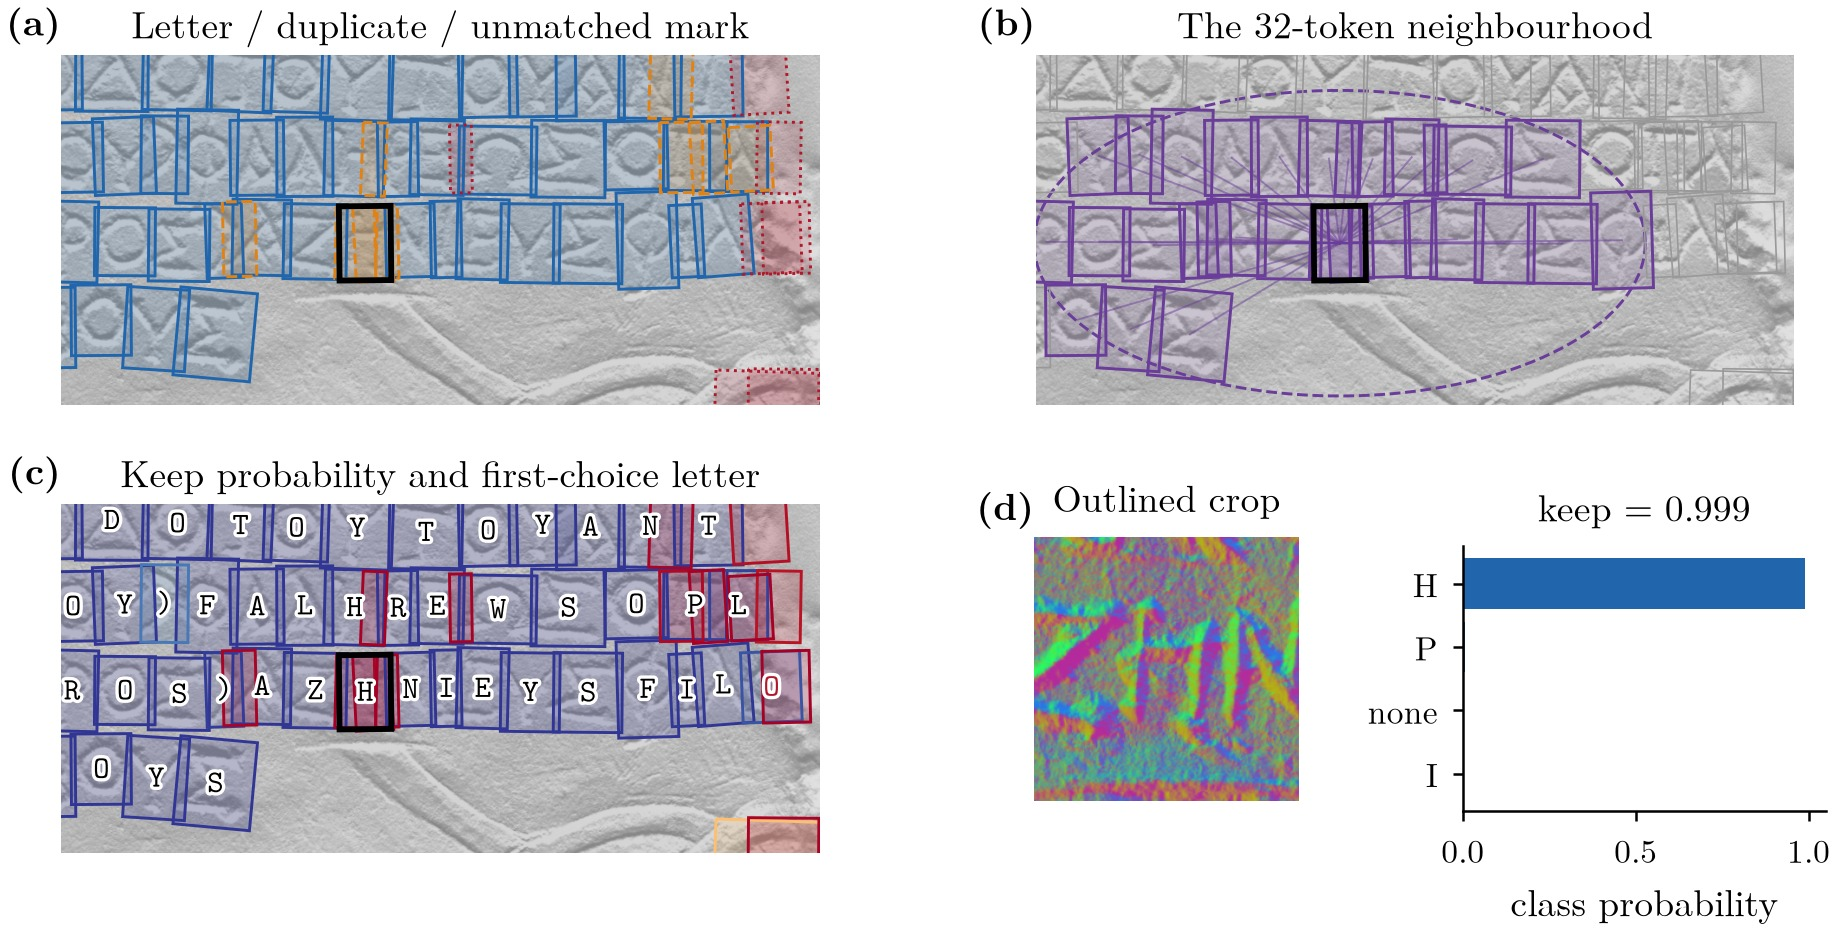
\includegraphics[width=\textwidth]{figs/neighbourhood.jpg}
\caption{\textbf{Reading a crop in its neighbourhood.} A region of \TeaserSqueeze{}; the black box marks
an annotated \code{\NeighbourhoodQuery{}}. (a)~Training labels distinguish letters, duplicate boxes and
unmatched marks. (b)~The 32 tokens available to this box, including itself. Lines join it to each
neighbour; learned attention weights are not drawn. (c)~Keep probabilities and first-choice letters; red
letters disagree with the training label. (d)~The outlined crop and its probabilities, including \none{}.}
\label{fig:neighbourhood}
\end{figure}

\subsection{How it learns rejection, duplication and context}
Training uses detected boxes, not perfect letter crops. Against the annotation of \Rone{}, a one-to-one
assignment first matches as many letters as possible at rotated IoU at least 0.3; ties prefer higher
calibrated detector probability, then higher IoU. A matched token takes its letter. All others take
\none{}, including extra boxes on a letter already claimed by another token. Rejection therefore means
\emph{this token should not emit an annotated letter}, not necessarily \emph{the paper contains no letter here}.

An extra classifier used only during training learns to read each crop on its own. It receives a letter
label for a one-to-one match at IoU at least 0.5, \none{} when the best overlap is below 0.3, and no label
between those thresholds. This gives the image encoder a direct learning signal.

The main reader must also learn to use context. We hide the crop description for 15\% of the tokens
being trained, replacing it with a learned placeholder while leaving their positions and neighbours
available. The crop-only classifier still sees the image; the main reader must work without it.
Only the main reader's contextual probabilities are used to produce transcripts.

\section{Training for changes in light and paper}
\label{sec:training}
A network trained on fixed crops could learn one lighting rig or one paper texture too closely. Training
therefore varies the relief itself as well as image brightness. We turn the virtual lights, change the
apparent depth and fade one view's contribution. Blur and noise alter the texture; small crop shifts and
flattened patches imitate imperfect centring and local damage. These transforms vary the image evidence;
they do not simulate how a squeeze is made. Appendix~\ref{app:recipe} gives their ranges.

The transforms keep a token's class and its page geometry unchanged. The page-wide lighting change is
shared within a training window; crop shifts and local damage vary between crops. Figure~\ref{fig:augmentation}
shows sampled versions of real crops.

\begin{figure}[t]
\centering
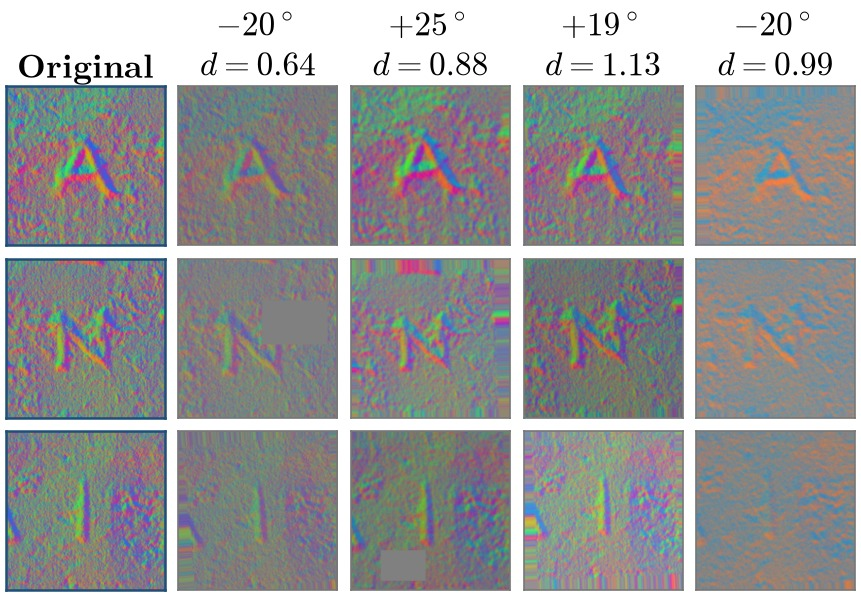
\includegraphics[width=\textwidth]{figs/augmentation.jpg}
\caption{\textbf{The same letter under different simulated conditions.} Three crops of public squeeze
IG\_II2\_493\_Copy1 and four sampled training versions of each. Headings give light rotation and depth
multiplier; blur, noise, shifts and local damage also vary.}
\label{fig:augmentation}
\end{figure}

Training uses windows of 384 nearby tokens. The nearest 192 contribute to the training error; the
others supply context. Two windows make one training step. The two readers train for 5 and 15
\emph{epochs}, or passes through the training data, and both use their final weights.
Optimiser settings are listed in Appendix~\ref{app:recipe}.

When producing a transcript, the network reads the whole page rather than training windows.
Each network sees five crop versions:
unchanged, rotated by $-2.5^\circ$ or $+2.5^\circ$, and scaled by 0.95 or 1.05. Geometry and neighbour
support stay fixed. The ten distributions are combined by averaging log probabilities and renormalising:
\begin{equation}
 \log P_i=\operatorname{log\,softmax}
      \left(\frac{1}{10}\sum_{r=1}^{10}\log P_i^{(r)}\right).
 \label{eq:combine}
\end{equation}
This is a normalised geometric mean of the ten distributions: a letter strongly opposed by one version is
penalised more than under an arithmetic average.

\begin{figure}[t]
\centering
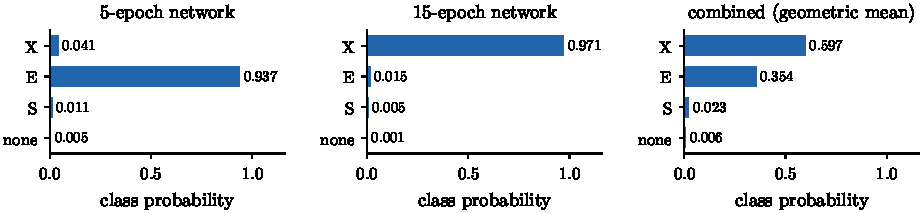
\includegraphics[width=\textwidth]{figs/tta.pdf}
\caption{\textbf{Combining probabilities, not first choices.} Token \TtaToken{} of \TeaserSqueeze{}.
The two networks favour \TtaFirstFive{} and \TtaFirstFifteen{}; their combination favours
\TtaFirstCombined{}. Each network's distribution already combines five crop views.
This is the most strongly disagreeing retained token among those with different first choices.
The four classes with greatest summed probability are shown.}
\label{fig:tta}
\end{figure}

\section{Recognition errors and confidence}
\label{sec:tokens}
Over the public set, the \TokensTokens{} tokens include \TokensClaims{} matched to an annotated letter
and \TokensNone{} assigned \none{}. At $k\ge0.5$, the reader keeps \TokensKept{}: it loses
\TokensLost{} matched letters (\TokensLostShare{}) and keeps \TokensSpurious{} unmatched tokens
(\TokensSpuriousShare{} of those kept). These counts describe individual boxes. Transcript errors also
depend on letter identity, reading order and row boundaries.

The keep probability separates matched letters from the rest better than the calibrated detector score
(Figure~\ref{fig:tokens}). It is close to observed
frequencies at the extremes but underestimates letter frequency in parts of the middle range. Consequently,
a probability such as 0.3 should not be treated as a guaranteed frequency, and thresholding at 0.5 loses
letters that search could still use.

Among tokens matched to letters, the correct identity ranks first for \TokensTopOne{}, and among the eight
letters offered to search for \TokensTopEight{}. Many mistakes are small changes in a worn stroke:
Α becomes Λ, Θ becomes Ο, or Δ becomes Α (Figure~\ref{fig:confusion}). The high top-eight rate motivates
keeping alternatives. It does not imply that the decoder knows which alternative is correct, nor include
letters with no proposal.

\begin{figure}[t]
\centering
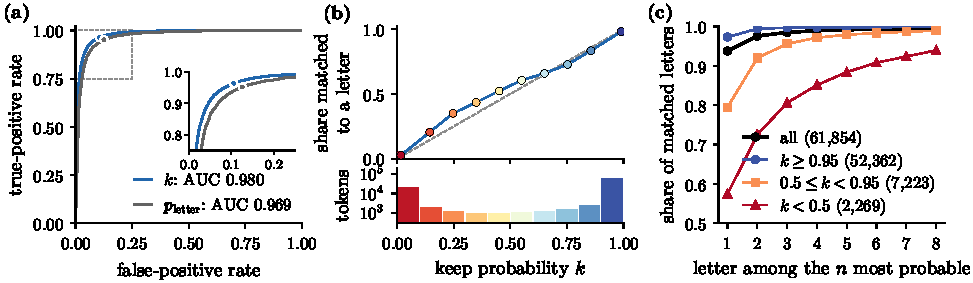
\includegraphics[width=\textwidth]{figs/tokens.pdf}
\caption{\textbf{Keeping a box and identifying its letter are different decisions.} All public tokens,
with each squeeze held out. (a)~True- versus false-positive rates as the threshold changes.
The area under the curve is \TokensAucKeep{} for the reader and \TokensAucDetector{} for the detector;
larger is better. Dots mark threshold 0.5. (b)~Observed match frequency against keep probability, with
counts below. (c)~The fraction of matched letters found among the top $n$ identities, excluding \none{}.}
\label{fig:tokens}
\end{figure}

\begin{figure}[t]
\centering
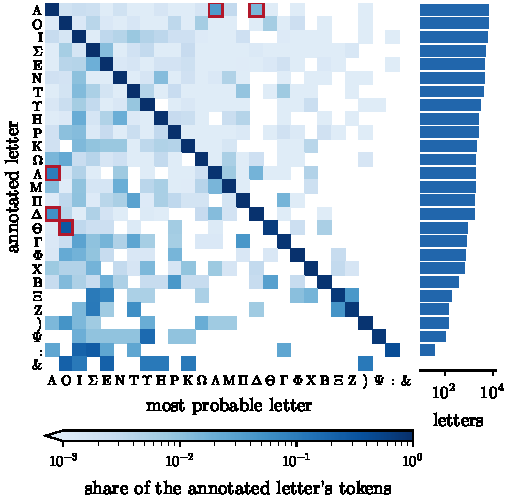
\includegraphics[width=0.78\textwidth]{figs/confusion.pdf}
\caption{\textbf{Which letters are confused?} The reader's first choice for \ConfusionTokens{} matched
public tokens, with letters in Greek. Each row is an annotated letter; each column is a predicted letter.
Colour shows the fraction within that row on a logarithmic scale; blank cells have no examples. The side
bars show letter counts. Boxes mark the five most frequent mistakes; \ConfusionTopTwoFrom{} becomes
\ConfusionTopTwoTo{} in \ConfusionTopTwoShare{} of matched \ConfusionTopTwoFrom{} tokens. Rejected boxes
are measured separately in Figure~\ref{fig:tokens}.}
\label{fig:confusion}
\end{figure}

\FloatBarrier
\section{Assembling rows and choosing their text}
\label{sec:decoder}
The page network has no transcript output. Its boxes must first be put into reading order. Tokens with
$k\ge0.5$ determine the page angle and are grouped by the organisers' version-2 row
procedure~\cite{trogs26data}. A token with $0.05\le k<0.5$ can join the nearest row if it lies within half
a letter height of the median baseline and within the row's span expanded by 2.5 letter heights at each
end. The others are omitted, including every
token below 0.05. Tokens within a row are ordered along the deskewed horizontal direction.

On the running squeeze, \RowsKept{} strong tokens form \RowsRows{} rows; \RowsWeakJoined{} weak tokens
join them, while \RowsWeakDropped{} join none (Figure~\ref{fig:rows}). The label and much of the ornament
are rejected before search. A wrong row grouping can nevertheless merge columns or break a curved row;
correct individual letters do not by themselves determine a correct transcript.

\begin{figure}[t]
\centering
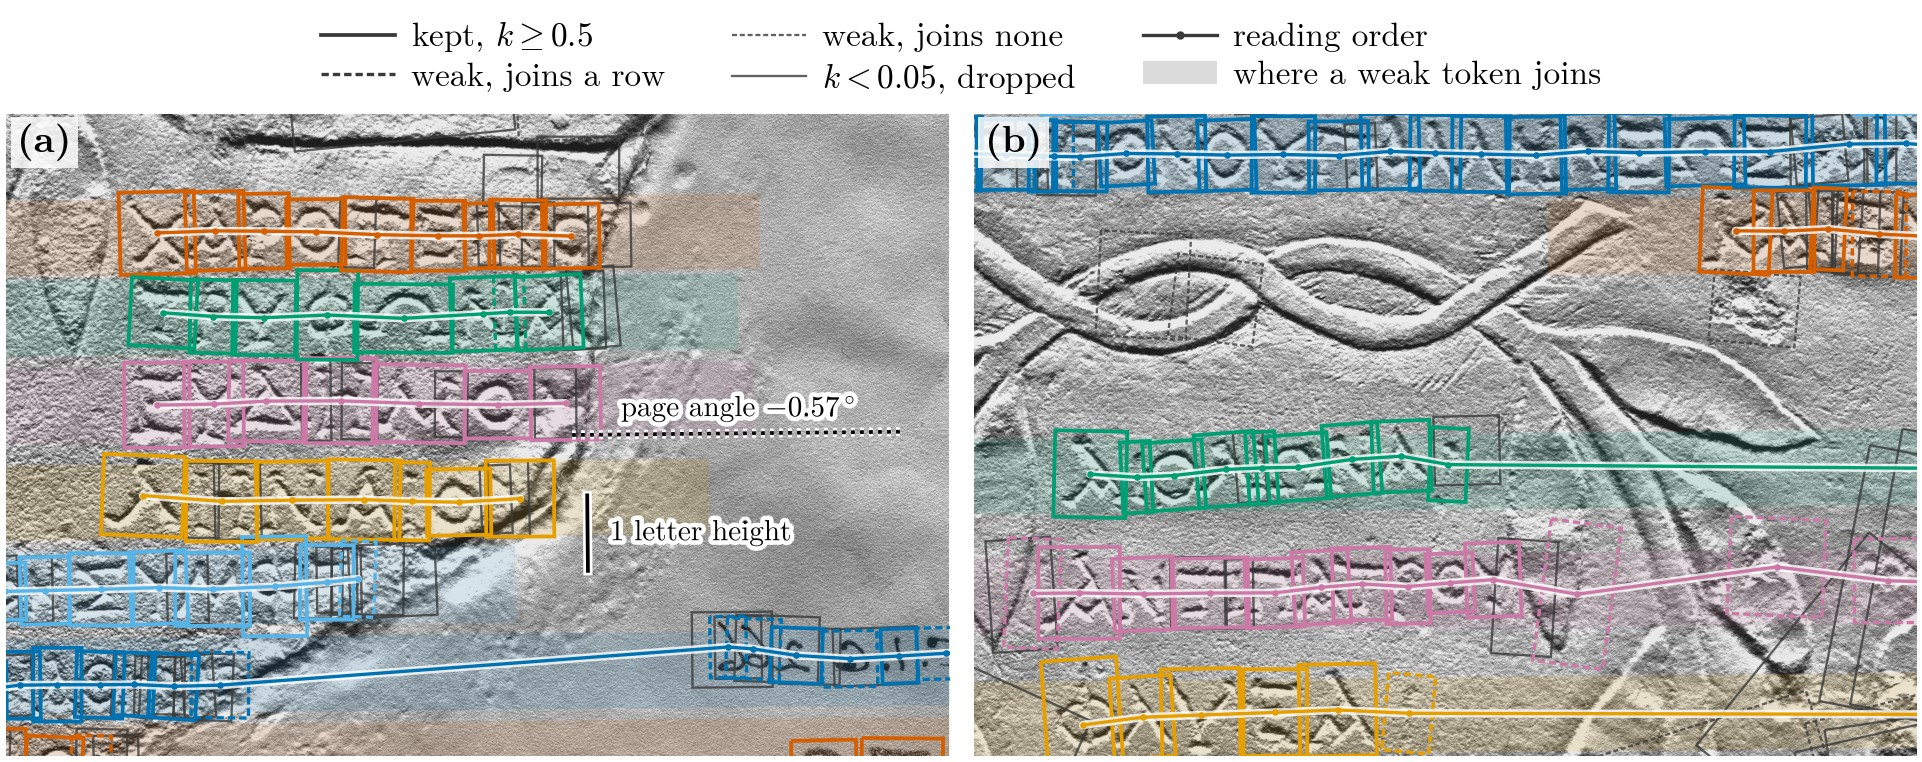
\includegraphics[width=\textwidth]{figs/rows.jpg}
\caption{\textbf{Where a weak mark is allowed to become a letter.} Two regions of \RowsBase{}.
Solid coloured boxes have $k\ge0.5$ and establish rows. Weak boxes joining a row are dashed in that row's
colour; weak boxes joining none are dashed grey, and boxes below 0.05 thin grey. Tinted bands show the
joining regions, and lines join tokens in reading order. These rows are built from the reader's outputs,
without the annotations. Even a weak mark can reach search if it lies on a strong row; an isolated weak
mark cannot.}
\label{fig:rows}
\end{figure}

\subsection{Comparing possible readings}
Each row position offers its eight most probable letters under $\pi_i$, and may be skipped if $k_i<0.95$.
For a candidate $y$ emitting positions $E$ from all row positions $T$, the final score is
\begin{equation}
\begin{split}
 S(y)={}&\underbrace{\sum_{i\in E}\log\pi_i(y_i)}_{\text{letter identity}}
 +w\underbrace{\left[\sum_{i\in E}\log k_i+
                         \sum_{i\in T\setminus E}\log(1-k_i)\right]}_{\text{emit or skip}}\\
 &+\lambda L(y)+\beta|y|.
\end{split}
\label{eq:score}
\end{equation}
The last terms are a character-model score and a per-letter bonus. The bonus counters the fact that adding
letters normally adds negative log probabilities. At $k_i\ge0.95$, emission is compulsory and the keep
term is set to zero. Elsewhere $k_i$ is clipped to $[10^{-4},1-10^{-4}]$ for stable logarithms.
The final weights are \DevScoreWeights{}.

The search proceeds left to right, keeping the 256 highest-scoring partial readings at each step
(\emph{beam search}). It runs at five settings of $(\lambda,w,\beta)$:
$(0,1,0)$, $(1,1,0)$, $(1,2,2.5)$, $(1,2,3.5)$ and $(1,3,3)$.
Their union gives a finite candidate pool, covering different compromises between letter identity,
retention and text plausibility. A later scorer can reorder this pool, but cannot expand it.
Search cannot recover a letter if no relevant token offers it among its top eight alternatives.

\subsection{Breaking context at gaps}
The median spacing of neighbouring strong tokens estimates the usual distance between letters.
If two consecutive emitted tokens stand more than 1.6 times that distance apart, the character models
start afresh. Thus a name before a broken stretch is not treated as directly adjoining a word after it.
This reset adds neither guessed letters nor a special symbol to the final transcript.
Row boundaries also restart context.

\section{Using Greek letter patterns}
\label{sec:lm}
\subsection{Patterns learned from existing texts}
Some letter sequences are more plausible in Greek than others. The character models estimate this
plausibility one letter at a time; they do not consult a dictionary of complete inscriptions.

The public row transcripts contain 62,246 letters. We count their short character sequences using
\emph{prediction by partial matching}, PPM-C~\cite{cleary1984,moffat1990}. The stored model supports
up to 11 preceding letters; decoding uses at most four. A second model, with up to five preceding letters,
is built from \ExtLetters{} million letters of openly licensed external Greek: Perseus, First1KGreek,
DDbDP, I.Sicily, IAph2007 and IOSPE (CC BY or CC BY-SA; manifests record URLs, licences and pinned
revisions). Before any counting or training, this text is decontaminated
(Section~\ref{sec:decontamination}).

PPM-C predicts from the counts following a given sequence. When those counts do not cover a letter,
it looks at a shorter sequence, excluding letters already accounted for; with no evidence left, it
uses a uniform distribution. The public and external predictions are mixed:
\begin{equation}
 P_{\mathrm{base}}(a\mid c)=(1-\omega)P_{\mathrm{public}}(a\mid c)+\omega P_{\mathrm{ext}}(a\mid c),
 \label{eq:base}
\end{equation}
with $\omega=\DevOpenWeight{}$ (Section~\ref{sec:results}). The public model excludes the fold being
evaluated. For test reading, it uses all 224 public squeezes.

\subsection{Removing the evaluated inscriptions from the external text}
\label{sec:decontamination}
External text can hold the inscriptions being evaluated: an edition of a squeeze among other inscriptions,
or a quotation of it in a literary text. The external text is therefore filtered against the transcripts of
all 274 annotated squeezes, the 224 public and the 50 TROGS-26 test squeezes, using every annotated letter
of both views. This is the one use of the test annotations: they decide which external text is removed
(Section~\ref{sec:results}).

A 15-letter sequence of a squeeze is \emph{rare} if at most \DeconRare{} external documents hold it.
A rare sequence is text of one inscription: its editions, copies and quotations. Formulae, titles and
common names recur in more documents and stay. An epigraphic document is taken to be a squeeze's
inscription if it holds at least \DeconDropAt{} distinct rare sequences of the squeeze, making up at least
\DeconShare{} of the sequences of the shorter of the two texts. These documents are removed whole:
\DeconDropped{}, found for \DeconPublicFound{} public and \DeconTestFound{} test squeezes. In every other
document, each occurrence of a rare sequence is cut out and its line split there, so neither the counts
nor the neural model's training windows hold it: \DeconCutLetters{} letters from \DeconCutDocuments{}
documents. A list naming the same person, or a decree repeating a clause, thus loses only the shared
stretch. A final scan finds no rare sequence of any squeeze in any remaining line.

Both thresholds were set on public squeezes only, by one measurement on the PHI Greek
inscriptions~\cite{phi}, which hold editions of most public squeezes under the IG numbers of their names.
PHI's terms do not allow redistribution; it is read for this measurement alone, and no model holds its
text. Counting documents over the open corpora and PHI's \DeconCalibPhiDocuments{} records together,
\DeconCalibShare{} of the sequences of a public squeeze found in a record citing its IG number
(\DeconCalibDocuments{} records of \DeconCalibSqueezes{} squeezes) occur in at most \DeconRare{}
documents; the rest are formulae. Of the \DeconCalibEditions{} records holding at least \DeconDropAt{} rare
sequences of their squeeze, none shares less than \DeconCalibShareMin{} of the shorter text. Without PHI,
no sequence is held by more documents, so every sequence rare in this measurement is rare in the filter.
Text that an evaluated inscription shares with more than \DeconRare{} other documents stays: it is as
available to a reader of any new inscription.

\subsection{Repetition on the same squeeze}
Names and formulae can repeat within one inscription even when uncommon elsewhere. A first pass selects
draft rows at $(\lambda,w,\beta)=(0.5,2,2)$. For each row, a temporary PPM-C model, called the \emph{page
cache}, counts sequences in the other draft rows, using up to four preceding letters and restarting at
gaps. The second pass uses
\begin{equation}
 P_{\mathrm{cachemix}}=0.8P_{\mathrm{base}}+0.2P_{\mathrm{other\ rows}}.
 \label{eq:cache}
\end{equation}
The row being read never supplies its own cache. This prevents direct self-counting, but errors can still
pass between rows: a mistaken draft repeated elsewhere can favour the same mistake. When there are no
other non-empty rows, no cache mixture is made.

\subsection{Using the letters on both sides}
A complete candidate can be scored using the letters after a doubtful character as well as those before
it. Forward and backward PPM models use the same corpora in opposite directions; cache mixtures are made
on both sides. For each gap-delimited run,
\begin{equation}
 L(y)=\sum_i\left[\log P_{\mathrm f}(y_i\mid y_{<i})+
                       \log P_{\mathrm b}(y_i\mid y_{>i})-
                       \log P_{\mathrm f}(y_i\mid\varnothing)\right].
 \label{eq:twosided}
\end{equation}
Subtracting the context-free term avoids counting a symbol's base preference twice. The sum serves only
to rank candidates and is not normalised over strings. The beam still proposes left to right; right
context enters when completed candidates are scored.

\subsection{Adding longer context}
A neural character model can use a longer stretch of preceding text: up to 192 symbols.
It first learns from the decontaminated external text, then receives further training on public transcript
rows mixed with external sequences. Training for a held-out fold excludes its transcripts; the test model
uses all public rows. Many training sequences start within a line, so the start symbol means that the
preceding text is unknown; a word need not begin there.

Only the forward term in the \emph{final} score changes:
\begin{equation}
 \log P_{\mathrm f}(a\mid c)\quad\longmapsto\quad
 \log\!\left[(1-\nu)P_{\mathrm f}(a\mid c)+\nu P_{\mathrm{neural}}(a\mid c)\right],
 \label{eq:neural}
\end{equation}
with $\nu=\DevNeuralWeight{}$ (Section~\ref{sec:results}). The backward and subtracted context-free terms
stay unchanged. The neural model supplies neither the
beams nor the draft rows for the cache. It reads each candidate run from a start symbol after every gap;
it can only choose a text already present in the finite visual candidate pool.

\subsection{The order of the passes}
Decoding a squeeze takes two search passes over its rows and one final choice:
\begin{enumerate}
\item \emph{Draft pass.} Beam search at the five settings of Section~\ref{sec:decoder}, with
$P_{\mathrm{base}}$, gives a candidate pool. Its best candidate under Eq.~\eqref{eq:score} at
$(\lambda,w,\beta)=(0.5,2,2)$, with the two-sided $L$ of Eq.~\eqref{eq:twosided} over $P_{\mathrm{base}}$,
is the row's draft.
\item \emph{Cache pass.} The other rows' drafts fill the page cache; beam search at the same five settings,
now with $P_{\mathrm{cachemix}}$, gives the row's final pool. A row whose other rows are all empty keeps
its draft pool.
\item \emph{Final choice.} Each candidate in the final pool is scored by Eq.~\eqref{eq:score} at
\DevScoreWeights{}, with the two-sided $L$ over the cache mixtures and its forward term mixed with the neural
model (Eq.~\eqref{eq:neural}). The best candidate is the row's text.
\end{enumerate}

\begin{figure}[t]
\centering
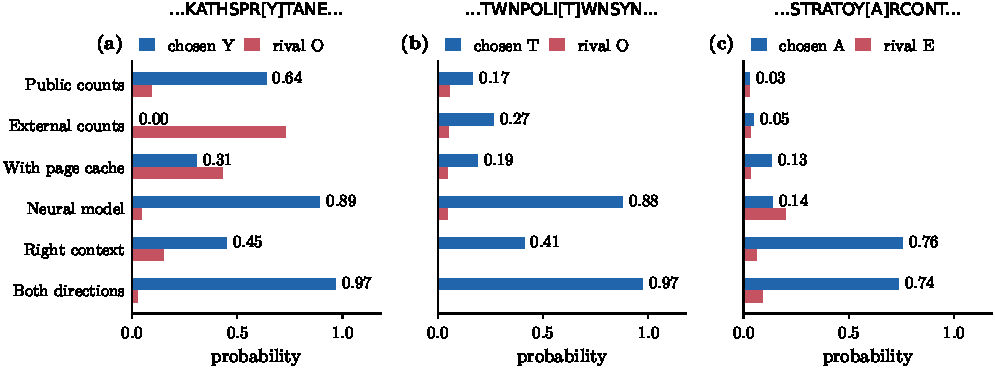
\includegraphics[width=\textwidth]{figs/lm_prior.pdf}
\caption{\textbf{What text context favours.} Three positions in public IG\_II2\_493\_Copy1, comparing
the chosen letter with one rival. Each stage adds one part of the adopted text model: external counts,
the page cache, the neural model and right-hand context, on top of the public counts; the six rows are
the same in all three panels. The two-sided
scores are normalised across letters for display. These plots measure text prediction alone; transcript
accuracy is measured in Section~\ref{sec:results}.}
\label{fig:lm}
\end{figure}

\begin{figure}[t]
\centering
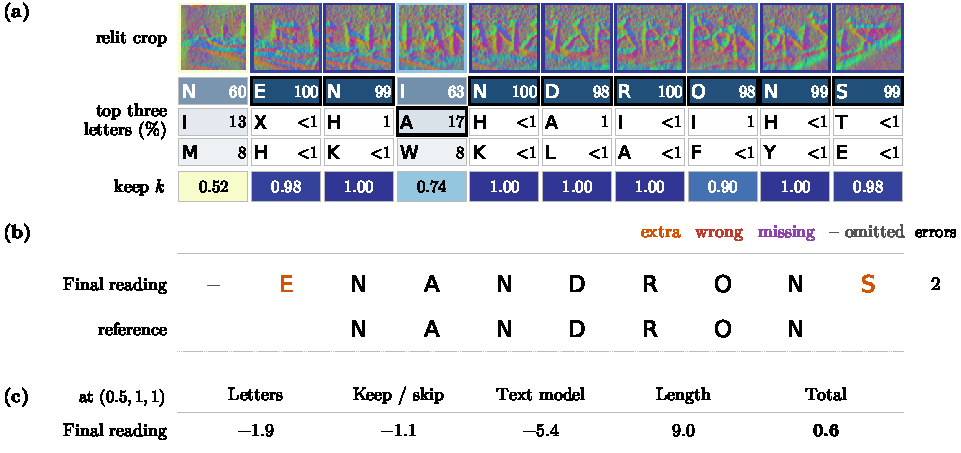
\includegraphics[width=\textwidth]{figs/lattice.pdf}
\caption{\textbf{Choosing a better reading, with errors still visible.} Row \LatticeRow{} of
\LatticeBase{}. (a)~Ten crops, their three most probable letters and keep probabilities. Boxes mark
the selected letters. (b)~The final reading and the reference.
The initial N is skipped and I changes to A; the extra E and S remain.
(c)~The parts of the final reading's score at the adopted weights \DevScoreWeights{}:
letters, keep/skip, text model and length. This example is a row of 10--25 positions.}
\label{fig:lattice}
\end{figure}

\section{Combining five readings}
\label{sec:rover}
The five fold detectors are different models. On a new squeeze they can propose different boxes,
estimate different scales and fit different registrations. At test time the \emph{same} 5- and 15-epoch
page networks, trained on all 224 public squeezes, read every chain's page. The five texts therefore
differ mainly through detection and alignment.

We combine the transcripts with ROVER~\cite{fiscus1997}. First, choose the transcript requiring the fewest
edits in total to match the other four. This is the \emph{pivot}. Align the other transcripts to it,
treating line breaks like other symbols. Then count the votes at each aligned position:
\begin{itemize}
\item The most frequent symbol wins. A gap counts as one vote, just like a letter.
\item A tie keeps the pivot's symbol.
\item A string inserted between pivot positions needs at least three identical votes and must beat
the votes for no insertion.
\end{itemize}
Winning gaps produce no character, and empty output rows are removed. The two highlighted positions
in Figure~\ref{fig:overview2} show a tie resolved by the pivot and a position removed by a gap vote.

Across the test squeezes, two chains' transcripts differ by an average of \RoverDistPP{} of the longer
transcript's length, measured by edit distance. The vote changes
\RoverChanged{} output characters relative to the pivot (\RoverSubstituted{} substitutions and
\RoverInsertionChars{} inserted characters) and removes \RoverRemoved{} pivot characters.
These changes measure disagreement between chains; a misreading shared by most chains survives the vote.

\section{How well it reads}
\label{sec:results}
\subsection{Public development and the fixed test output}
There are 224 public squeezes: 181 training, 22 validation and 21 internal-test. The five detectors train
on the 181 training squeezes only, each without its own fold; validation and internal-test pages are held
out from every detector. Reader folds have sizes 45, 45, 45, 45 and 44, each containing its corresponding
detector fold plus eight or nine additional public squeezes. A public squeeze is therefore read by a
detector that did not train on it, and by the reader pair, public language model and neural fine-tune that
exclude its entire reader fold. The pair reads through the map selected on the images
(Section~\ref{sec:registration}), although its training crops were cut through the map fitted to detected
letter centres. The pair that reads the test pages trains in the same way on all 224 public squeezes.

For each reported fold, the weights of the text models and of the decoder are selected using the other
four folds over \DevGridPoints{} points: the external weight $\omega\in\{\DevOpenWeights{}\}$,
$\lambda\in\{0.3,0.4,0.5,0.65,0.8,1.03\}$, $w\in\{1,2,3,4\}$, $\beta\in\{0,1,2,3,4\}$ and the neural
weight $\nu\in\{0.5,0.6,0.7,0.8,0.9\}$. This keeps each fold out of its own weight selection; the public
rates of Table~\ref{tab:results} read each fold at its own choice. The point with the fewest errors over
all five folds, $\omega=\DevOpenWeight{}$ and \DevCombo{}, is the one used on the test pages
(Figure~\ref{fig:sweep}); it lies at the largest external weight of the grid.
The choice made without a fold matches it in \DevNestedAgree{} of the five folds; over all folds it makes
\DevOofErrors{}/\DevOofChars{} errors (\DevOofCer{}), a figure selected on those same squeezes.
Other choices are shared by all folds. The architecture and training variation were developed using
public results, and the detector epoch was chosen once, on fold~0; the public estimate is not an
independent test of those choices.

The organisers' version-2 scorer~\cite{trogs26data} compares one output transcript with each annotated
view and reports three rates. Core CER counts edit operations against confident letters, including
row-boundary characters; rows with no confident letters are omitted. All CER counts them against every
annotated letter. Opt CER lets uncertain letters be omitted at no cost; an uncertain letter read correctly
joins the reference count. Missing, substituted and inserted letters, and row splits or merges, all cost.
We sum errors and reference characters over both views, rather than averaging per-squeeze percentages.
All counts in Table~\ref{tab:results} follow that definition.

% Written by paper/make_results.py from the run outputs; do not edit.
\begin{table}[htbp]\centering
\begin{tabular}{@{}lrrr@{}}\toprule
Evaluation set & Errors & Characters & Core \cer{} \\\midrule
Public (224 squeezes) & 12{,}612 & 131{,}473 & \textbf{9.59\%} \\
\quad Without \code{Merged} (208) & 7{,}935 & 96{,}628 & 8.21\% \\
\quad No related squeeze in another fold (176) & 10{,}631 & 105{,}068 & 10.12\% \\
TROGS-26 test (50 squeezes) & 1{,}464 & 15{,}862 & \textbf{9.23\%} \\\bottomrule
\end{tabular}
\caption{\textbf{Character error rates against both annotated views.} Public squeezes use one held-out chain each, and each fold is read at the weights chosen on the other four; test squeezes use readers trained on all public data and a vote over five chains. Public fold rates (0--4): 8.73\%, 9.92\%, 12.87\%, 9.01\%, 6.95\%.}
\label{tab:results}
\end{table}


The ROVER transcripts of the 50 TROGS-26 test squeezes~\cite{trogs26data} were frozen before the reported
final evaluation. It gives \DevTrogsErrors{}/\DevTrogsChars{} Core errors (\DevTrogsCer{}), All CER
\DevTrogsAllErrors{}/\DevTrogsAllChars{} (\DevTrogsAllCer{}), and Opt CER
\DevTrogsOptErrors{}/\DevTrogsOptChars{} (\DevTrogsOptCer{}).
All counts include both annotation views, with a prediction for every squeeze.
Transcript hashes were recorded with the score, and no model, setting or transcript changed in response to
that evaluation. Test labels entered one step, the decontamination of the external text
(Section~\ref{sec:decontamination}): they decided which external text was removed before training. Otherwise
no test label entered training, the folds or parameter selection.

\begin{figure}[t]
\centering
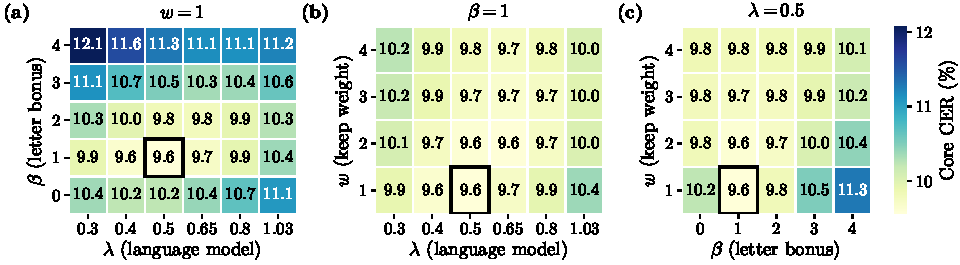
\includegraphics[width=\textwidth]{figs/sweep.pdf}
\caption{\textbf{What the decoding weights change.} Three slices of the public grid through the selected
point, at its external and neural weights: (a)~language-model weight and letter bonus; (b)~language-model
and keep weights; (c)~letter bonus and keep weight. Cells show Core CER (\%), rounded to one decimal place.
Each setting chooses among saved candidate readings; it does not run the visual models again.
Each held-out fold chooses its weights using the other folds; \DevNestedAgree{} of the five select the
boxed point. The plotted cells themselves are pooled over all public squeezes, for diagnosis.}
\label{fig:sweep}
\end{figure}

\subsection{The average hides difficult squeezes}
The public median per-squeeze Core CER is \SqueezesMedianCer{}, below the pooled \DevOofCer{}. The
\SqueezesWorstCount{} worst public squeezes account for \SqueezesWorstErrorShare{} of the errors in
\SqueezesWorstCharShare{} of the reference characters. The 208 squeezes without \code{Merged} in their
names make \DevNoMergedErrors{}/\DevNoMergedChars{} errors (\DevNoMergedCer{}); this subset is reported
alongside the full benchmark. The 50 test squeezes range from \TrogsLowestCer{} to
\TrogsHighestCer{}, with median \TrogsMedianCer{} (Figure~\ref{fig:squeezes}).

\begin{figure}[t]
\centering
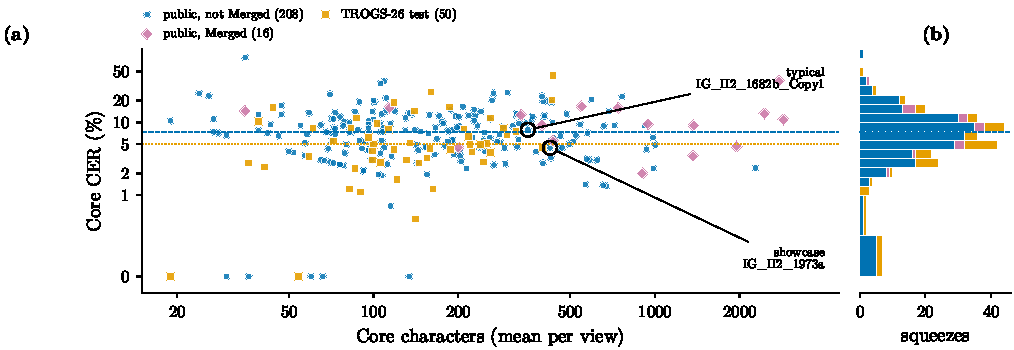
\includegraphics[width=\textwidth]{figs/squeezes.pdf}
\caption{\textbf{Some inscriptions are much harder than others.} (a)~Each public and test squeeze's
Core CER against its mean reference length per view. Public points are split by the filename marker
\code{Merged}; test points use the frozen five-chain score. Lines mark public and test medians.
(b)~Counts of squeezes in error-rate bands. CER axes are linear below 1\% and logarithmic above it, so true
zero-error cases are retained rather than shifted to an artificial floor.}
\label{fig:squeezes}
\end{figure}

\subsection{A complete example}
The running squeeze is useful for showing ornament and crops, but is easier than average. For a fuller
error example, we select the public squeeze with 150--450 Core characters in \Rone{} whose pooled CER
is nearest the median within that size range: \ExampleBase{} (\SqueezesTypicalCer{}).
Figure~\ref{fig:example} shows every row. Its \Rone{} comparison has
\ExampleErrors{} errors in \ExampleChars{} characters. Lost letters occur at row starts and ends as well as
inside words, and some rows begin with a letter the reference lacks. The annotations, proposal set, reader
and row search all constrain what can be read; the language model has not completed the words to familiar
forms.

\begin{figure}[htbp]
\centering
\begin{minipage}[c]{0.25\textwidth}
 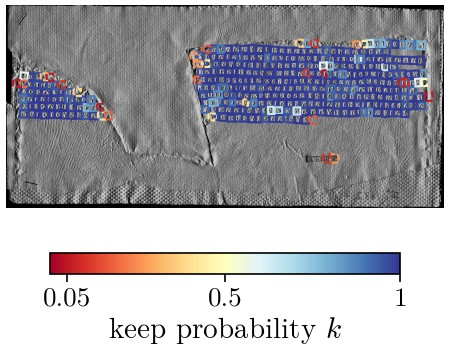
\includegraphics[width=\linewidth]{figs/example.jpg}
\end{minipage}\hfill
\begin{minipage}[c]{0.71\textwidth}
 \centering\small\fitwidth{\ExampleRows}
\end{minipage}
\caption{\textbf{A complete transcript and its errors.} Held-out public squeeze \ExampleBase{}, selected
by the size-and-median rule in the text. Left: boxes available to the decoder (solid strong, dashed weak).
Right: the \Rone{} Core reference and system output. Red marks substitutions, purple missing letters,
and orange extra letters; all are underlined. An output row without a reference number is extra.
The \ExampleErrors{} errors include row-boundary edits.}
\label{fig:example}
\end{figure}

\FloatBarrier
\section{Limits of the reading}
\label{sec:limits}
A missed proposal is irrecoverable. A letter below keep 0.05, or a weak token outside every strong row,
is lost before character-model scoring. A mistaken row order can mix columns even when every crop is
legible. Each context block of the page network sees only a local neighbourhood; repetition elsewhere on the
page reaches the decoder through the draft rows, which can repeat errors as readily as names.

Relief recovery fails where shadows do not behave like directional slopes, scans cover different paper,
or registration fails at a seam. Local agreement weighting limits contamination but cannot recover a
stroke hidden from the remaining light. The three virtual channels re-present two measured slopes: they
add no observation and recover no absolute surface depth.

A high keep probability can also protect a wrong mark. At or above 0.95, search cannot skip it; below that,
a large skip cost may still outweigh a text-model penalty. Conversely, a visible letter omitted from a
confident-letter reference can count as an insertion. The training labels teach the network to
match annotation decisions as well as letter shapes. Neither visual plausibility nor agreement among
five related chains proves a reading correct. The transcript is a proposed reading to check against the
photographs, not a restoration or a scholarly edition of the inscription.

\clearpage
\appendix
\section{Implementation details}
\label{app:recipe}
\subsection{Alignment and detection}
\label{app:align}
Across the 224 public squeezes, the number with at least 98\% of annotated letter correspondences within a
quarter letter height rises from \RegPassOld{} for the centre fit to \RegPassNew{} for the selected map
(Figure~\ref{fig:registration}c). The rule of Section~\ref{sec:detector} repeats detection on 18 public
squeezes and on 52 of the 250 test-chain records (five chains for each of 50 test squeezes).
Table~\ref{tab:recipe} lists the registration search.

\subsection{The page network}
The image encoder has 12 layers of width 384, six attention heads, a class token, four register tokens
and $14\times14$ image patches. The class token $c_i$ and mean patch token $\bar z_i$ (excluding registers)
form a 384-dimensional crop encoding $e_i$. The 18 measured features $f_i$ are standardised using
training-fold statistics, then embedded and added:
\begin{equation}
 e_i=\operatorname{LN}\bigl(W_e[c_i;\bar z_i]\bigr),\qquad
 x_i^{(0)}=e_i+W_2\operatorname{GELU}(W_1 f_i).
 \label{eq:embed}
\end{equation}
LN denotes layer normalisation and GELU the activation function.
The neighbourhood $N(i)$ contains the 32 nearest tokens, including $i$, under
$\Delta u^2+(2\Delta v)^2$, where $u$ runs along rows and $v$ across them in letter heights.
For attention head $\eta$, the weight on neighbour $j$ is
\begin{equation}
 \omega_{ij}^{\eta}=\operatorname*{softmax}_{j\in N(i)}
 \left(\frac{q_i^\eta\cdot k_j^\eta}{\sqrt{64}}+B(f_{ij})_\eta\right),
 \qquad B:\mathbb R^8\to\mathbb R^{64}\to\mathbb R^6.
 \label{eq:attention}
\end{equation}
Here $q_i^\eta$ and $k_j^\eta$ are learned query and key vectors, distinct from the keep probability
$k_i$; $f_{ij}$ contains the eight pair measurements in Table~\ref{tab:features}.
Four blocks combine the six heads, with residual connections and a $384\to1536\to384$ feed-forward
network. The output is $P_i=\operatorname{softmax}(W_h\operatorname{LN}(x_i^{(4)}))$.
The reader has about 29.2 million parameters: 21.6 million in the image encoder and 7.1 million in the
context blocks.

\begin{table}[htbp]
\centering\small
\begin{tabular}{@{}lp{0.73\textwidth}@{}}
\toprule
Input & Measurements \\
\midrule
Detection (5) & Logit of calibrated probability; fused score; scores from the three renderings \\
Box shape (5) & Log height, width and aspect ratio; sine and cosine of twice the box's relative tilt \\
Overlap (3) & Maximum IoU; maximum IoU with a more probable neighbour; log overlap count \\
Page (5) & Log letter height in pixels; log token count; confident-token fraction; single-view flag;
registration inlier share \\
Token pair (8) & Along-row and across-row displacement; log distance; IoU; log height and width ratios;
probability-logit difference; self indicator \\
\bottomrule
\end{tabular}
\caption{\textbf{Measurements supplied with each crop.} Positions and sizes use letter heights in a
page frame rotated to the estimated text direction. Overlap features use the 16 nearest boxes,
approximated as rectangles in that frame.
The page angle is estimated from detections before reading, then re-estimated from keep probabilities
when forming rows.}
\label{tab:features}
\end{table}

\subsection{Training objective and settings}
With core tokens $C$ and auxiliary-labelled core tokens $R$, the training loss is
\begin{equation}
 \mathcal L=\frac{1}{|C|}\sum_{i\in C}-\log P_i(t_i)
       +\frac{0.5}{|R|}\sum_{i\in R}-\log P_i^{\mathrm{read}}(t_i^{\mathrm{read}}).
 \label{eq:loss}
\end{equation}
Here $t_i$ is token $i$'s training label, a letter or \none{}, and $t_i^{\mathrm{read}}$ its label for the
crop-only classifier, whose probabilities are $P_i^{\mathrm{read}}$ (Section~\ref{sec:pagenet}).
Context tokens outside the core also propagate gradients through their crops. Two windows are
accumulated per optimiser step. AdamW uses learning rates $5\cdot10^{-5}$ for the encoder and
$5\cdot10^{-4}$ for the rest, weight decay 0.05, 5\% linear warm-up and cosine decay.
The 15-epoch reader uses encoder stochastic depth 0.1; neither reader selects a checkpoint on a
reader-validation split. The separate neural character model has about 14.25 million parameters.

The relief transforms turn the virtual lights by up to $30^\circ$, scale each gradient component
within $\exp(\pm0.2)$, and fade one component in 30\% of training windows. Apparent depth ranges from
0.6 to 1.3 times its original value, blur reaches one pixel and noise 0.02. Each crop can move by
4\% of its side; with probability 0.15, a rectangle covering 3--12\% is flattened.

\begin{table}[htbp]
\centering\small
\begin{tabular}{@{}lp{0.70\textwidth}@{}}
\toprule
Component & Fixed settings \\
\midrule
Registration & Phase correlation over quarter turns and small angular offsets; ECC Euclidean, then
affine. Local levels: tiles of 12, 6 and 6 letter heights with displacement limits of 5, 1.5 and 0.5
letter heights; thin-plate spline smoothed until orientation-preserving. Median tile correlation selects
one of three maps. \\
Detector & YOLO26-L OBB; 100-epoch schedule, epoch 59 used. Chain~0 chooses the best
held-out mAP$_{50:95}$ epoch; the same epoch is used for all chains. Detailed inference: 40-pixel letter
height, 1280-pixel tiles, 25\% overlap; one-to-many detection head with rotated NMS at IoU 0.8 within
each tile. Across the three images, weighted box fusion at IoU 0.55, then Gaussian soft-NMS. \\
Crop encoder & DINOv3 ViT-S/16, 12 layers, width 384, six heads; class token plus mean of 196 patch
tokens, projected $768\to384$ with layer normalisation. \\
Page blocks & Four pre-LN blocks, six heads of width 64, 32-token support; pair-bias MLP
$8\to64\to6$ per block; feed-forward $384\to1536\to384$; dropout 0.1. \\
Reader training & 384-token windows, 192-token core, two windows per step; mask probability 0.15;
auxiliary loss weight 0.5; AdamW, bf16, gradient-norm clip 1. Final checkpoints at 5 and 15 epochs. \\
Crop augmentation & Rotation $\pm5^\circ$, scale 0.9--1.1; brightness gain parameter 0.2 and bias
parameter 0.08, each multiplied by a draw in $[-0.5,0.5]$, plus the relief transforms above. No flips. \\
Neural text base & Eight layers, width 384, six heads, context 192, tied embeddings; 6,000 steps,
512 sequences per step, AdamW peak $6\cdot10^{-4}$, 500 warm-up steps, cosine decay; every 200th
external line held out. 80\% of sampled sequences start inside a line. \\
Neural fine-tune & 100 steps; per step 64 transcript rows and 64 external sequences, their losses
averaged; AdamW at $10^{-4}$. Fold-specific transcript exclusions; all-public model for test. \\
Final selection & Width-256 beams, eight letters per token; gap restart at 1.6 pitches; cache
0.8/0.2; external weight $\omega=\DevOpenWeight{}$; \DevCombo{}. \\
\bottomrule
\end{tabular}
\caption{Settings that determine the computation. Training labels and the two distinct matching thresholds
are described in Section~\ref{sec:pagenet}; evaluation and selection boundaries are in
Section~\ref{sec:results}.}
\label{tab:recipe}
\end{table}

\FloatBarrier
\section{Sources and reproduction}
\label{app:external}
The adopted inference configuration is \path{configs/pagenet_only_style_neural.json}. It resolves the
image-registration/detect-again path, the two all-public mild-style readers, two-sided character models,
and the neural forward mixture; \path{configs/pagenet_only_style_neural_oof.json} applies it to the
public folds, each read by the pair trained on the other four. Reader training recipes are
\path{configs/style_mild_5_epochs.json} and \path{configs/style_mild_15_epochs.json}; public folds are
\path{data/folds_public224.json}. The code and configurations are at
\url{https://github.com/ppdms/greek_squeezes_e2e}. The trained models are public at
\url{https://huggingface.co/buckets/papadimas/greek_squeezes} in the \code{trogs26/} namespace,
with a checksum manifest (\code{MANIFEST.sha256}).

The code follows the stages described in the report:
\begin{itemize}[nosep,beginpenalty=10000,midpenalty=10000]
\raggedright
\item Alignment and detection: \path{trogs26/registration_images.py} and
\path{trogs26/detect/redetect.py}.
\item Relief and crops: \path{trogs26/relief.py} and \path{trogs26/dino/crops.py}.
\item Reading, text models and search: \path{trogs26/pagenet/}, \path{trogs26/lm/} and
\path{trogs26/decode/}.
\item Transcript voting: \path{trogs26/rover.py}.
\end{itemize}
The reader jobs are \path{gcp/jobs/pagenet_fold.sh} (a fold's networks), \path{gcp/jobs/pagenet_all.sh} (the
networks trained on all 224) and \path{gcp/jobs/pagenet_images_read.sh} (reads through the registration chosen on
the images, of the public folds or of new pages).
The character-model training job is \path{gcp/jobs/neural_lm.sh}.
For a new split, \code{python -m trogs26.decode.newpages} runs variant \code{P} with the adopted
configuration; \code{python -m trogs26.rover} combines its five chain transcripts.
\path{paper/data/trogs26_score.json} preserves the resolved
configuration, the 50 prediction hashes, per-squeeze counts and final totals from the fixed-output score.
The paper generators reuse those counts; they read no test annotation and run no scorer.

\paragraph{Figure provenance.}
\path{paper/make_figures.py} writes the figures and their numerical labels to \path{paper/figs/}, except
the diagram of the page network (Figure~\ref{fig:pagenet}). It is drawn by hand in TikZ
(\path{paper/diagram/pagenet.tex}) around the crops and first-choice letters of Figure~\ref{fig:overview2},
stage~6; its neighbourhood is a schematic page.
Detector, token, row and error plots use the
current public out-of-fold records, with the 18 detect-again records substituted where required.
The main specimen is \code{IG\_II2\_1973a}; the complete error example is selected by the stated
size-and-median rule. Saved public assets from \code{IG\_II2\_493\_Copy1} supply the augmentation draws
and page pictures; \path{paper/decode_assets.py} recomputes their decode and letter-model distributions
under the final system. The neighbourhood picture shows geometric support only. ROVER examples
use test \emph{outputs} only. \path{paper/make_results.py} writes the
result macros and table from stored sweeps and the frozen score. LuaLaTeX builds this manuscript with
\code{latexmk -pdf report.tex}. Neither figure generation nor manuscript compilation runs a
page network or the test scorer.

\section*{Acknowledgments}
The image encoder uses Meta AI's DINOv3 pretrained weights under the DINOv3 License. The detector uses
Ultralytics YOLO26. We thank the TROGS organisers for the photographs, annotations and evaluation tools,
and the open Greek text projects for their corpora and explicit licences.

\begin{thebibliography}{99}\footnotesize\setlength{\itemsep}{0pt}
\bibitem{howe2025} Howe, N.R., Chang, F., Falbo, I., Brown, T., Hershkowitz, A.: Character recognition for Greek
squeezes. International Journal on Document Analysis and Recognition 28(3), 345--356 (2025).
\url{https://doi.org/10.1007/s10032-025-00540-y}
\bibitem{trogs26data} Hershkowitz, A., Howe, N., Cosgrove, B., Brown, T.: TROGS-26 test images, with
annotations and version-2 evaluation code. Data, Smith College, Northampton, MA (2026).
\url{https://scholarworks.smith.edu/dds_data/19}
\bibitem{simeoni2025} Sim\'eoni, O., et al.: DINOv3. arXiv:2508.10104 (2025).
\bibitem{yolo26} Jocher, G., Qiu, J., Liu, M., Lyu, S., Akyon, F.C., Kalfaoglu, M.E.: Ultralytics YOLO26:
unified real-time end-to-end vision models. arXiv:2606.03748 (2026). Software:
\url{https://github.com/ultralytics/ultralytics}.
\bibitem{bookstein1989} Bookstein, F.L.: Principal warps: thin-plate splines and the decomposition of deformations.
IEEE TPAMI 11(6), 567--585 (1989). \url{https://doi.org/10.1109/34.24792}
\bibitem{evangelidis2008} Evangelidis, G.D., Psarakis, E.Z.: Parametric image alignment using enhanced correlation
coefficient maximization. IEEE TPAMI 30(10), 1858--1865 (2008). \url{https://doi.org/10.1109/TPAMI.2008.113}
\bibitem{solovyev2021} Solovyev, R., Wang, W., Gabruseva, T.: Weighted boxes fusion: ensembling boxes from different
object detection models. Image and Vision Computing 107, 104117 (2021).
\url{https://doi.org/10.1016/j.imavis.2021.104117}
\bibitem{bodla2017} Bodla, N., Singh, B., Chellappa, R., Davis, L.S.: Soft-NMS---improving object detection with
one line of code. In: ICCV, pp.~5562--5570 (2017). \url{https://doi.org/10.1109/ICCV.2017.593}
\bibitem{zadrozny2002} Zadrozny, B., Elkan, C.: Transforming classifier scores into accurate multiclass probability
estimates. In: KDD, pp.~694--699 (2002). \url{https://doi.org/10.1145/775047.775151}
\bibitem{cleary1984} Cleary, J.G., Witten, I.H.: Data compression using adaptive coding and partial string matching.
IEEE Transactions on Communications 32(4), 396--402 (1984). \url{https://doi.org/10.1109/TCOM.1984.1096090}
\bibitem{moffat1990} Moffat, A.: Implementing the PPM data compression scheme. IEEE Transactions on Communications
38(11), 1917--1921 (1990). \url{https://doi.org/10.1109/26.61469}
\bibitem{fiscus1997} Fiscus, J.G.: A post-processing system to yield reduced word error rates: Recognizer output
voting error reduction (ROVER). In: IEEE ASRU, pp.~347--354 (1997). \url{https://doi.org/10.1109/ASRU.1997.659110}
\bibitem{phi} The Packard Humanities Institute: Searchable Greek Inscriptions.
\url{https://inscriptions.packhum.org}
\end{thebibliography}
\end{document}
